% !TEX root = /Users/Gela/Desktop/Thesis_latex/thesis.tex


\section{Flowchart investigation}
Two different setups for a comparing system to the current system were investigated, section \ref{Flowchart}, and System 2 were chosen to be the comparing system. Both Systems were considered fulfilling most of the requirements, section \ref{framing}, for an updated version. \\

In order to choose one comparing system benefits and disadvantages with the two system were investigated. \\

System 1, figure \ref{fig:FlowCInves1}, is considered capable of creating a high pressure drop over the membrane. The hypothesis is also that it is capable of creating the biggest pressure drop with the least amount of energy needed. A disadvantage is considered  that implementing a pump in the purified water path will increase the risk that the pump may release particles into purified water which is, from a patient safety perspective, a high risk factor. \\

System 2, figure \ref{fig:Sys2}, is considered capable of creating a high pressure drop over the membrane. It is also capable of controlling the recovery factor which, due to theory increases the membrane life time and performance. It might also be capable of minimize the salt concentration close to membrane surface area if increasing recirculation flow, e.g, create turbulence close to the membrane surface. \\


The two comparing systems were set to:\\
\begin{figure}[h]
\centering
\begin{minipage}{.5\textwidth}
    \centering
    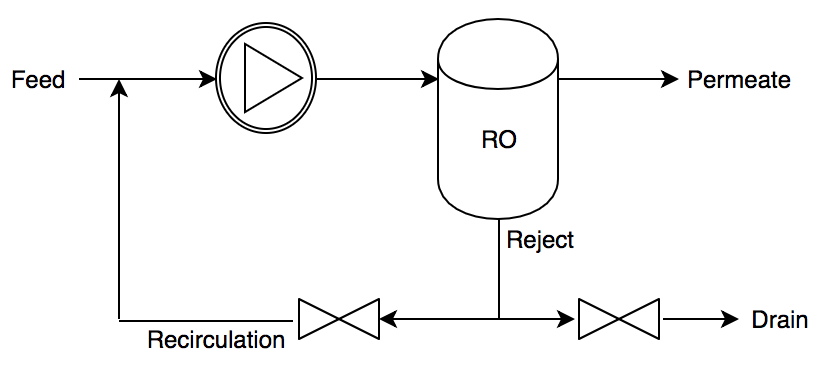
\includegraphics[width=0.8\textwidth]{Sys1}
    \caption{Current System}
    \label{fig:System1}
\end{minipage}%
\begin{minipage}{.5\textwidth}
  \centering
  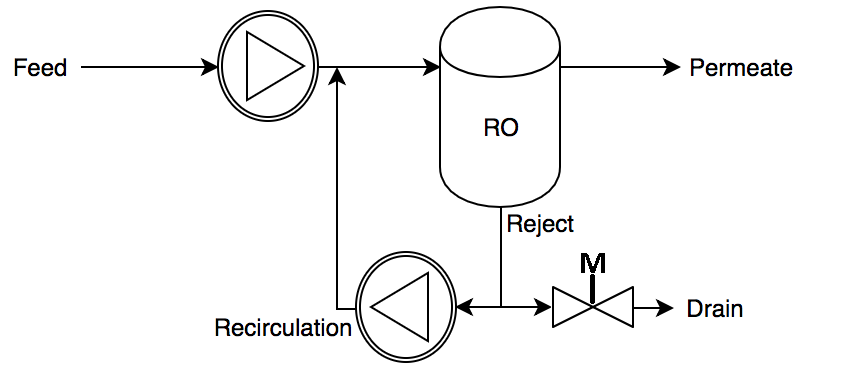
\includegraphics[width=.8\linewidth]{Sys2}
  \caption{System 2}
  \label{fig:System2}
\end{minipage}
\end{figure}

\newpage

\section{Investigation}
\subsection{Current system}

Temperature, feed pressure and feed water conductivity were the three main factors that was identified to have a significant impact on the performance of the membrane. However, testing was needed to conclude how much and in what way these parameters affect the membrane. The goal of the first round of tests was to investigate how much these parameters affected the current one pump system. 
The system was specified to be able to operate from 20 to 40 degrees celsius and from 300 to 3000 uS/cm in the recirculation loop. A simple controller was implemented to run the feed pump at 60\% if the conductivity was lower than 1000 uS/cm and increase the pump to 80\% if the conductivtity was higher than 1000 uS/cm.  
To be able to determine the impact of changes in these parameters three tests were needed. A fixed temperature was maintained with a heating bath and by increasing the conductivity in the bath from 280 uS/cm to 3000 uS/cm and varying the pump speed from 60 \% to 80\% it was possible to simulate how the membrane performed within the operating range. Eight steady states were investigated in each test according to the test plan. The system logged all signals during the test and the data could be analyzed to determine how all interesting parameters were affected during the different steady states.


\begin{table}[H]
\centering
\begin{tabular}{|p{1.4cm}||p{2cm}|p{3.2cm}|p{1.8cm}|}
 \hline
 \textbf{Steady state }&Temperature&Feed Conductivity&Motor effect \\
 \hline
 1.1 & 18 $^\circ$C   & 280 \SI{}{\micro\siemens} & 60 \% \\
 1.2   &  18 $^\circ$C   & 500 \SI{}{\micro\siemens} & 60 \% \\
 1.3 &  18 $^\circ$C  &1000 \SI{}{\micro\siemens} & 60 \% \\
 1.4 &  18 $^\circ$C  &1000 \SI{}{\micro\siemens} & \textbf{80 \%} \\
 1.5 &18 $^\circ$C &2000 \SI{}{\micro\siemens}& 60 \%\\
 1.6 &18 $^\circ$C  &2000 \SI{}{\micro\siemens}& \textbf{80 \%}\\
 1.7   &18 $^\circ$C & 3000 \SI{}{\micro\siemens}&60 \% \\
 1.8   &18 $^\circ$C&3000 \SI{}{\micro\siemens}& \textbf{80 \%}\\
 \hline
 2.1 & 30 $^\circ$C & 280 \SI{}{\micro\siemens}&60 \%\\
 2.2 & 30 $^\circ$C &500 \SI{}{\micro\siemens}& 60 \%\\
 2.3 & 30 $^\circ$C&1000 \SI{}{\micro\siemens}& 60 \%\\
 2.4 & 30 $^\circ$C&1000 \SI{}{\micro\siemens}& \textbf{80 \%}\\
 2.5 & 30 $^\circ$C&2000 \SI{}{\micro\siemens}& 60 \%\\
 2.6 & 30 $^\circ$C&2000 \SI{}{\micro\siemens}& \textbf{80 \%}\\
 2.7 & 30 $^\circ$C& 3000 \SI{}{\micro\siemens}&60 \%\\
 2.8 & 30 $^\circ$C& 3000 \SI{}{\micro\siemens}&\textbf{80 \%}\\
 \hline 
 3.1 & 40 $^\circ$C& 280 \SI{}{\micro\siemens}& 60 \%\\
 3.2 & 40 $^\circ$C &500 \SI{}{\micro\siemens}& 60 \%\\
 3.3 & 40 $^\circ$C  & 1000 \SI{}{\micro\siemens}& 60 \%\\
 3.4 & 40 $^\circ$C  & 1000 \SI{}{\micro\siemens}& \textbf{80 \%}\\
 3.5 & 40 $^\circ$C&2000 \SI{}{\micro\siemens}& 60 \%\\
 3.6 & 40 $^\circ$C &2000 \SI{}{\micro\siemens}& \textbf{80 \%}\\
 3.7 & 40$^\circ$C &3000 \SI{}{\micro\siemens}& 60 \%\\
 3.8 & 40$^\circ$C &3000 \SI{}{\micro\siemens}& \textbf{80 \%}\\
\hline
\end{tabular}
\caption{Testcases}
    \label{tab:testcases} 
\end{table}

\newpage
Test number one was split up in two parts. First the heating bath was set to 18 degrees and the feed pump was set to 60 \%. Thereafter, the conductivity in the tank was adjusted to 280 uS/cm and increased in steps to 3000 uS/cm. The graph below show an overview of the test.

\begin{figure}[H]
    \centering
    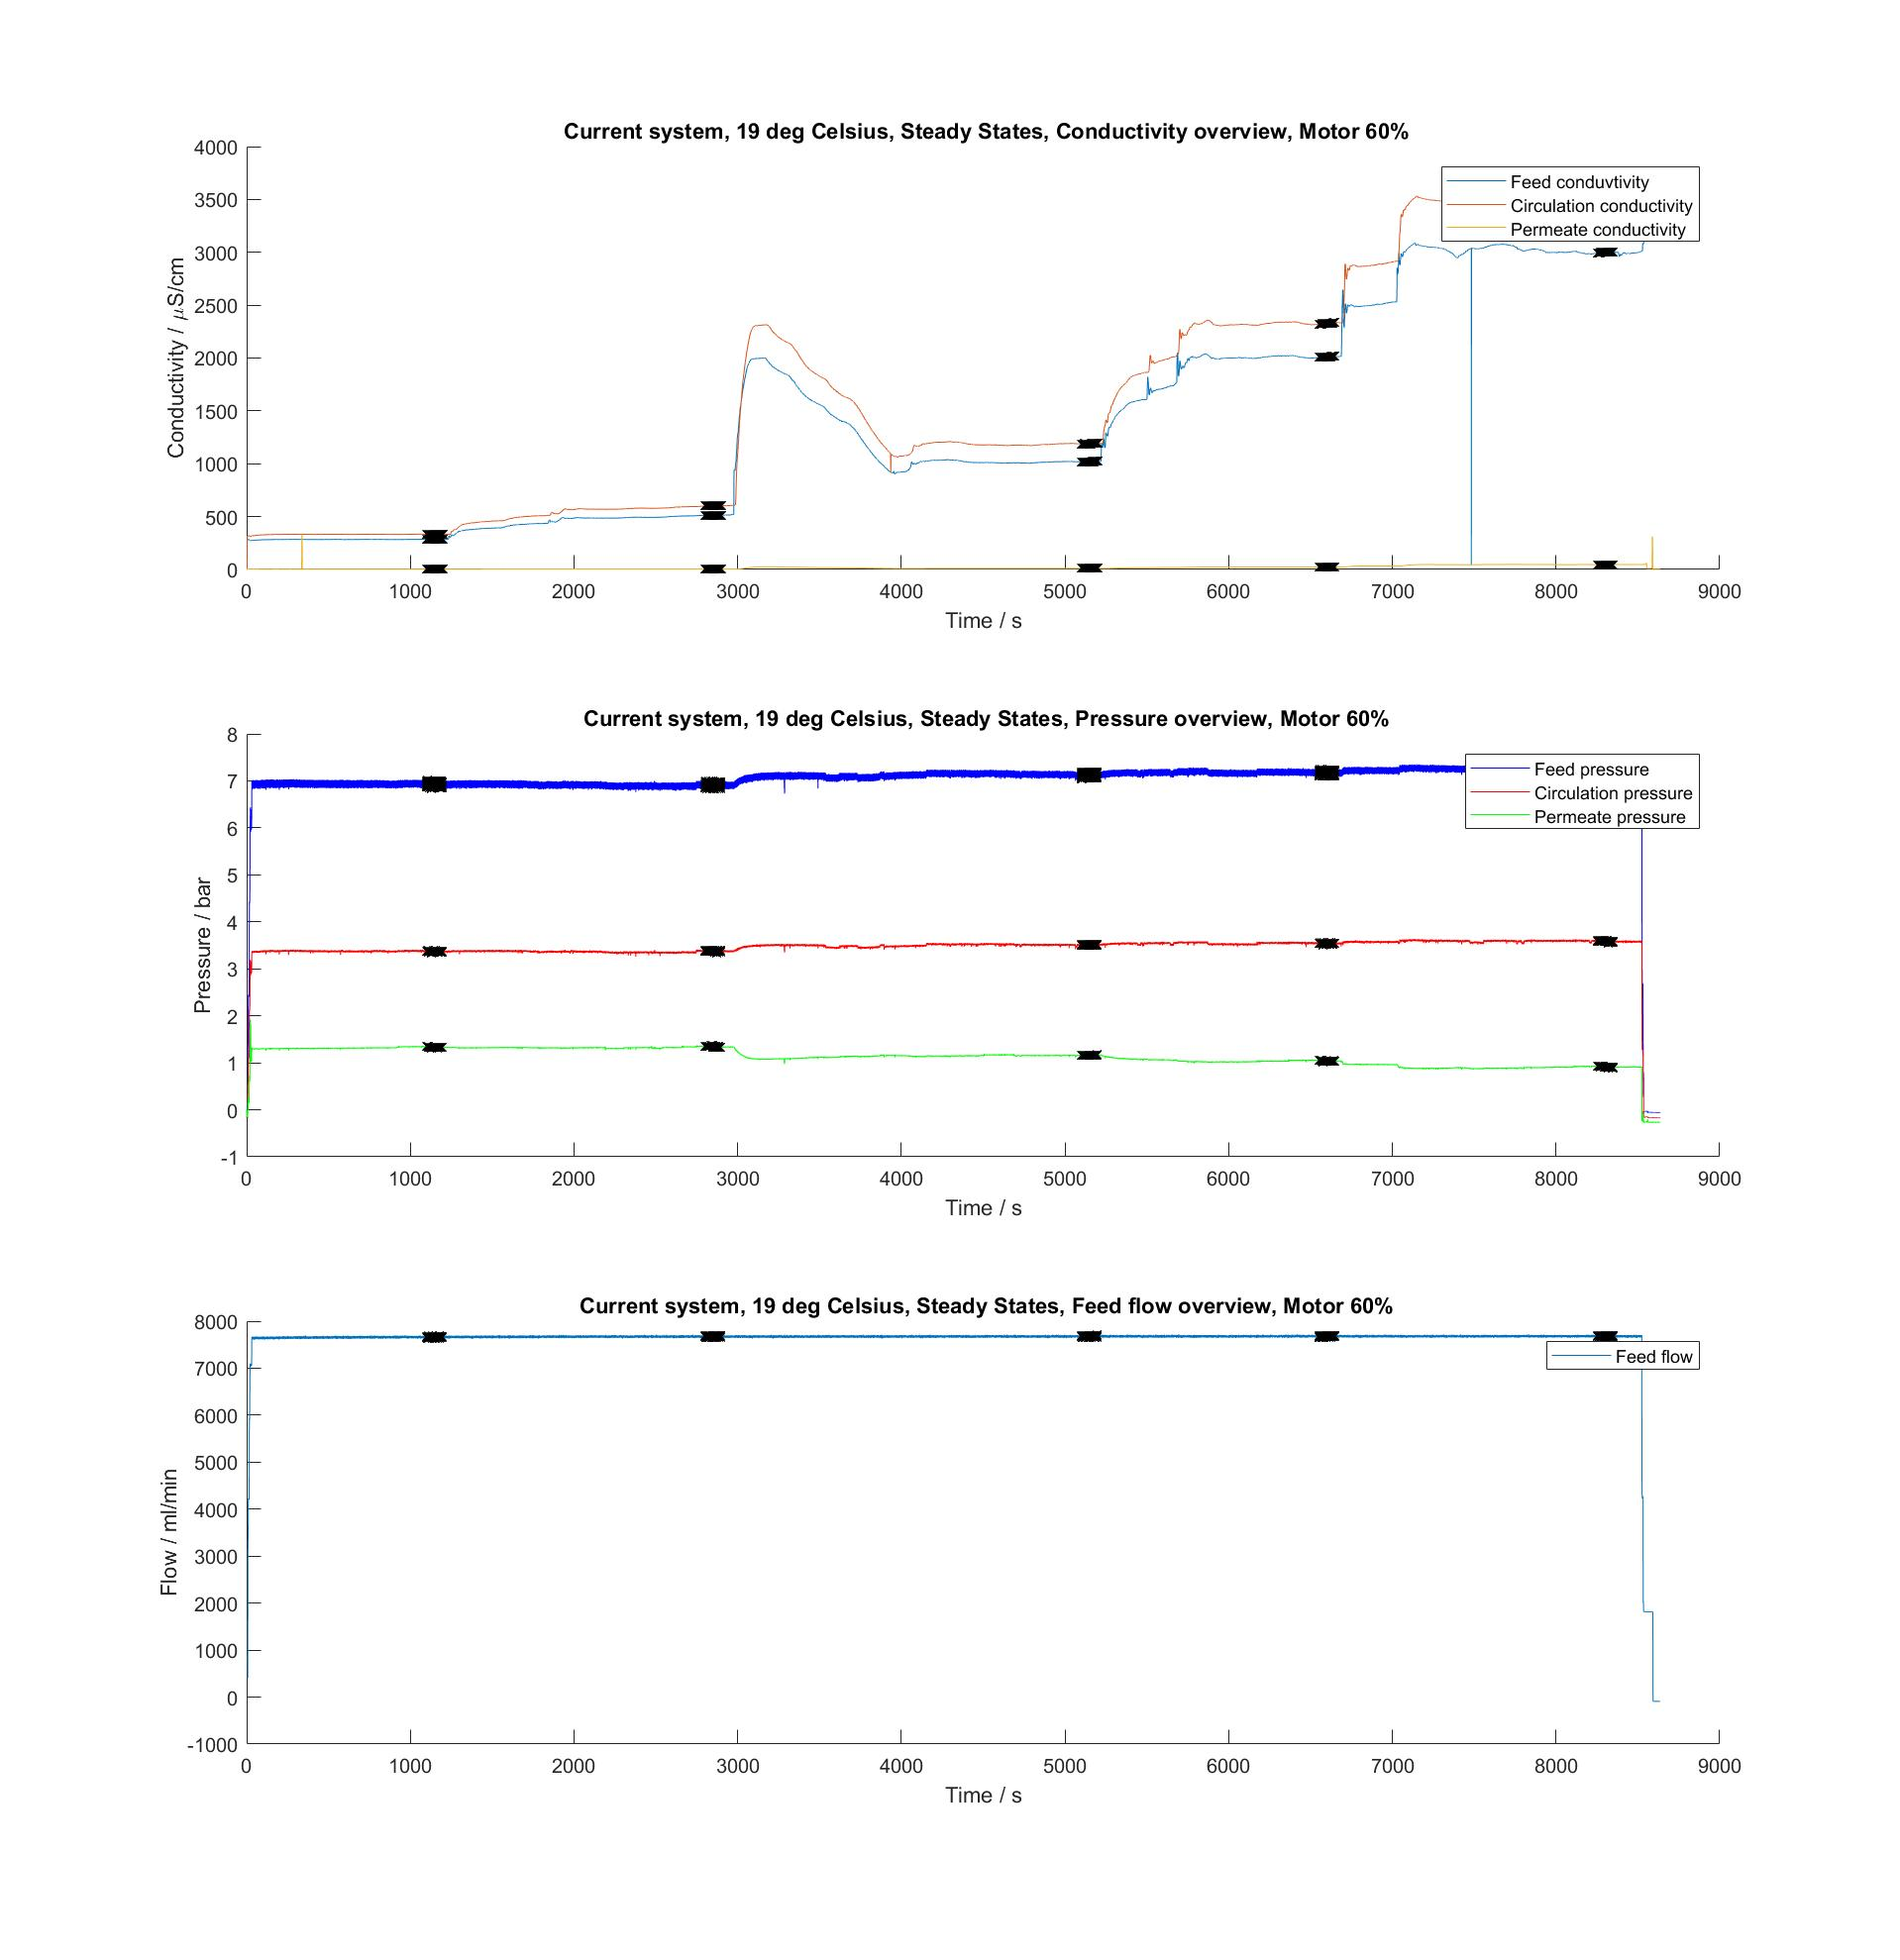
\includegraphics[width=1.1\textwidth]{overview20_60}
    \caption{Test 1, Current system, 18 degrees celsius. Steady states 1.1, 1.2, 1.3, 1.5 and 1.7 }
    \label{fig:PressConn}
\end{figure}

\newpage

The second part of the first test was carried out with the pump running at 80\%. In this test the conductivity was decreased from 3000 uS/cm to 280 uS/cm.
  
\begin{figure}[H]
    \centering
    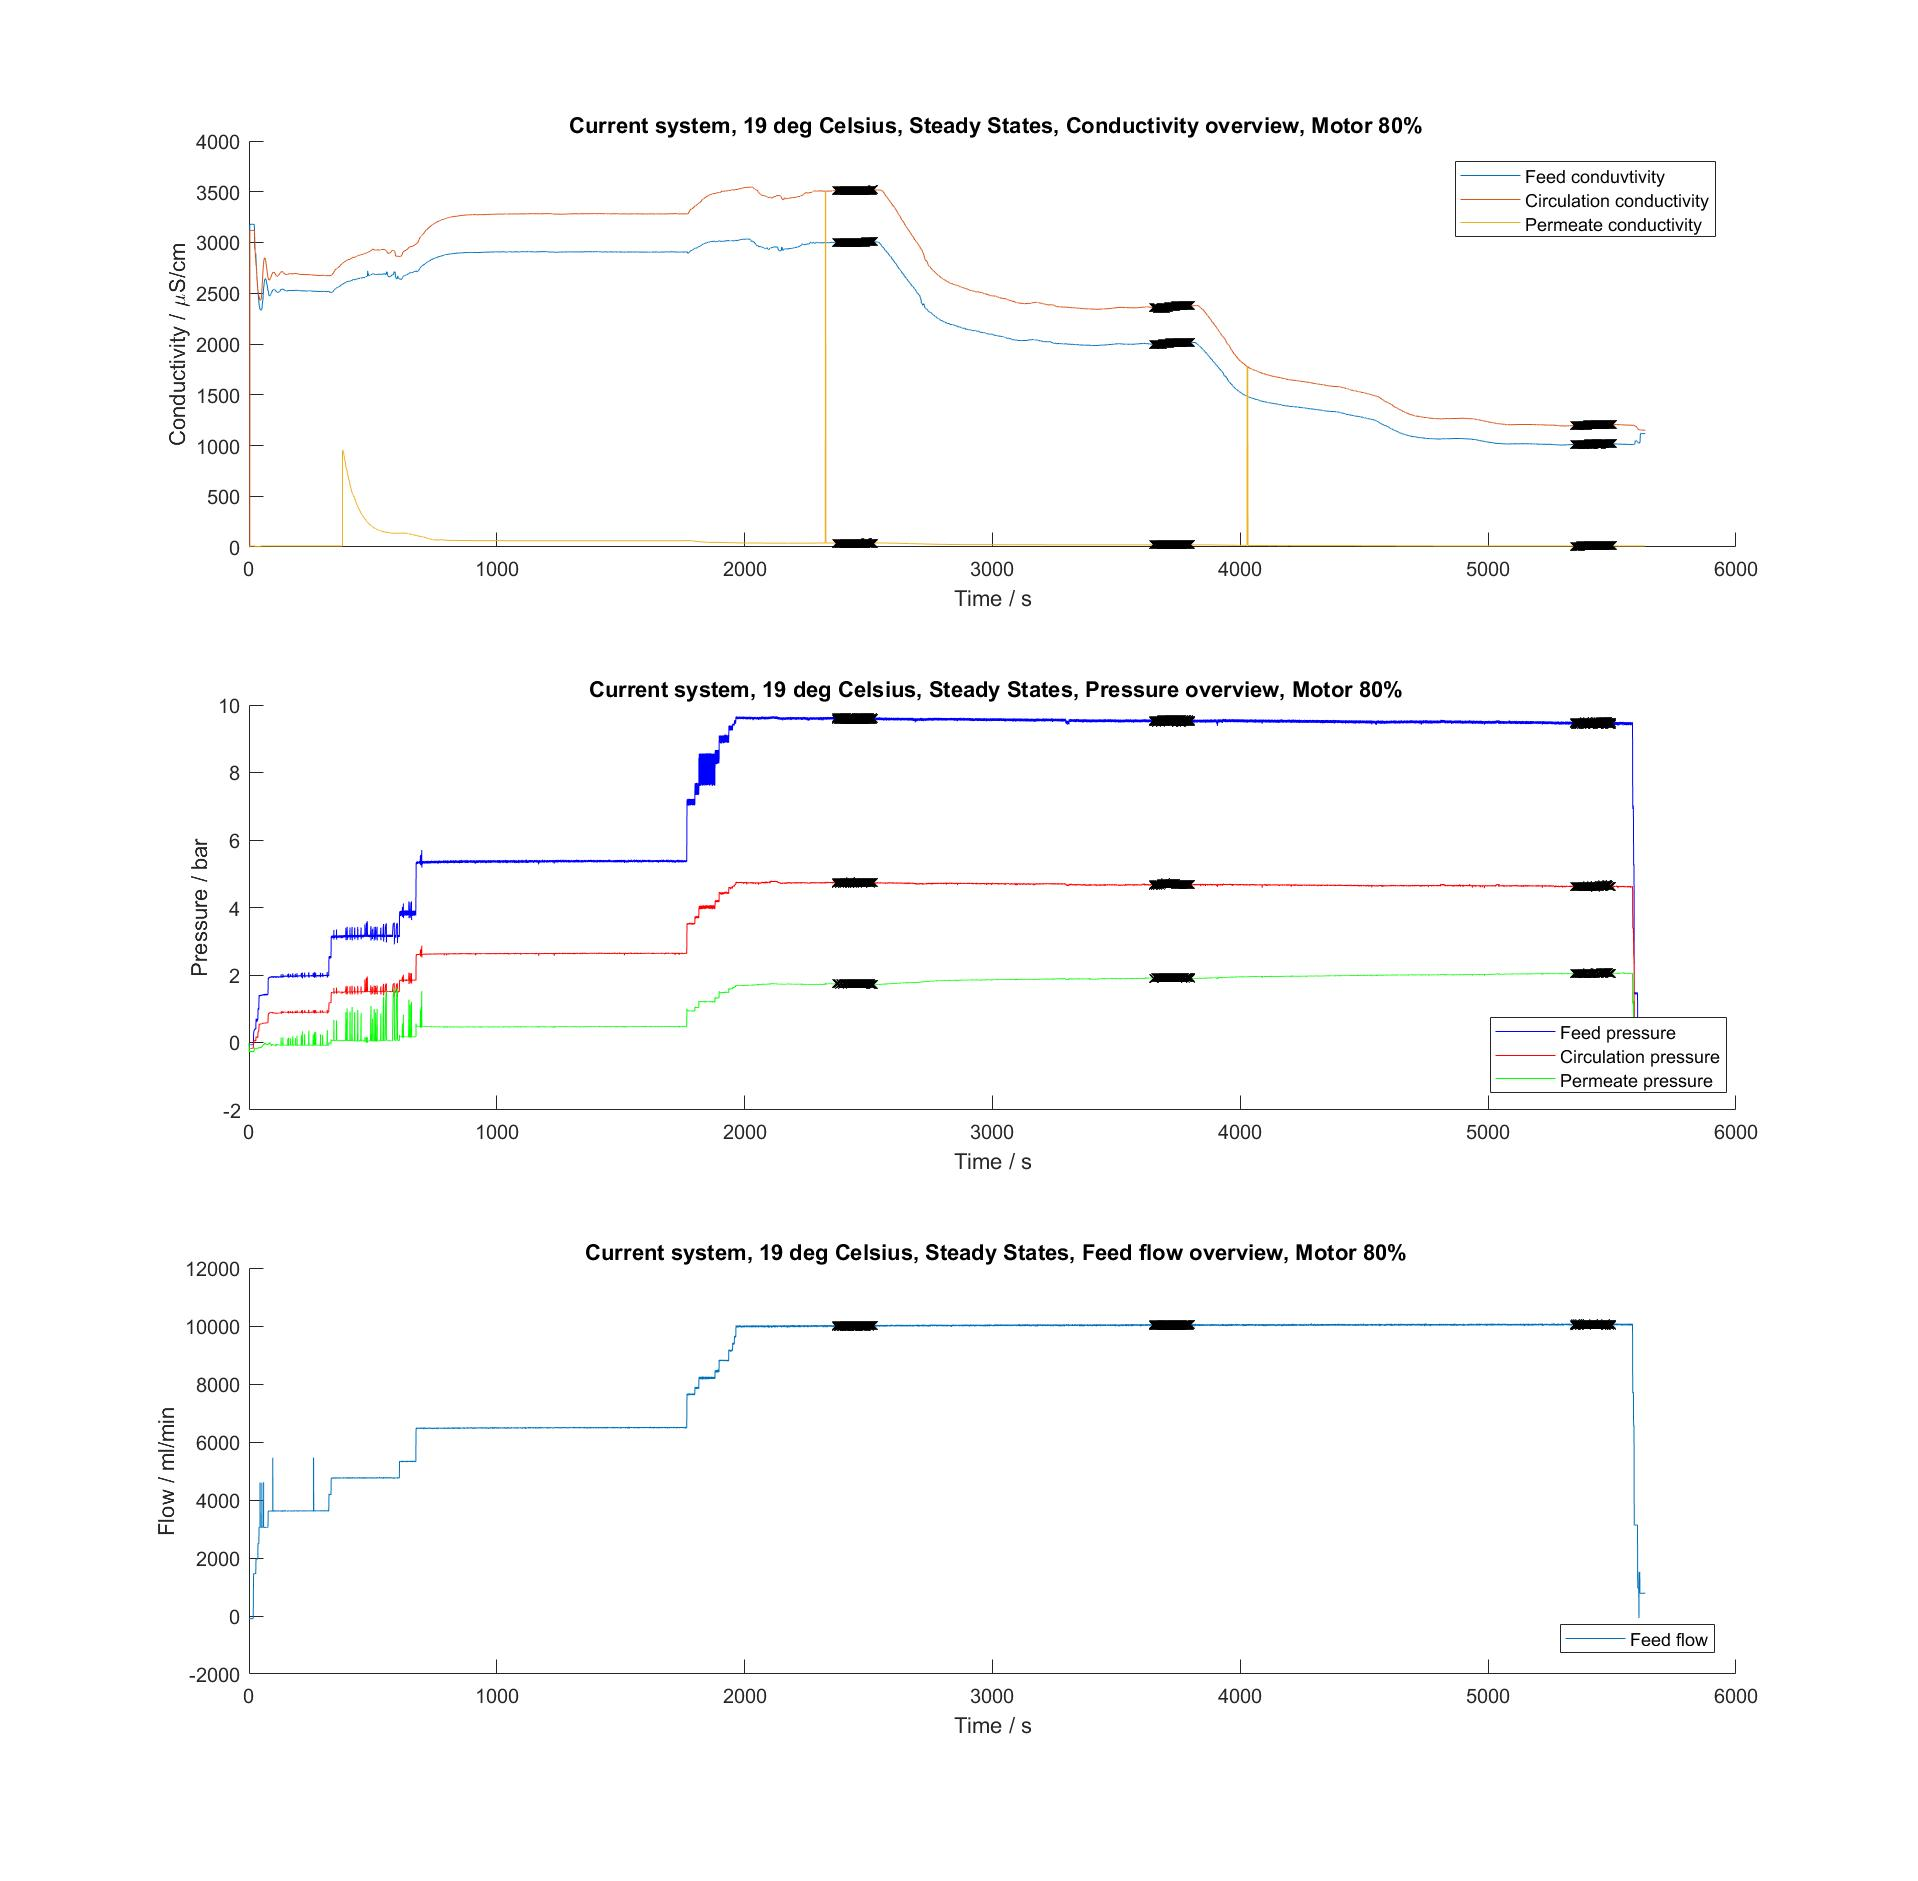
\includegraphics[width=1.1\textwidth]{overview20_80}
    \caption{Test 1, Current system, 18 degrees celsius. Steady states 1.4, 1.6 and 1.8}
    \label{fig:PressConn}
\end{figure}

\newpage

By post post-procesing the data from test one in Matlab it was possible to visually show how the system parameters were affected by the changed pump speed and feed conductivity. 

\begin{figure}[H]
    \centering
    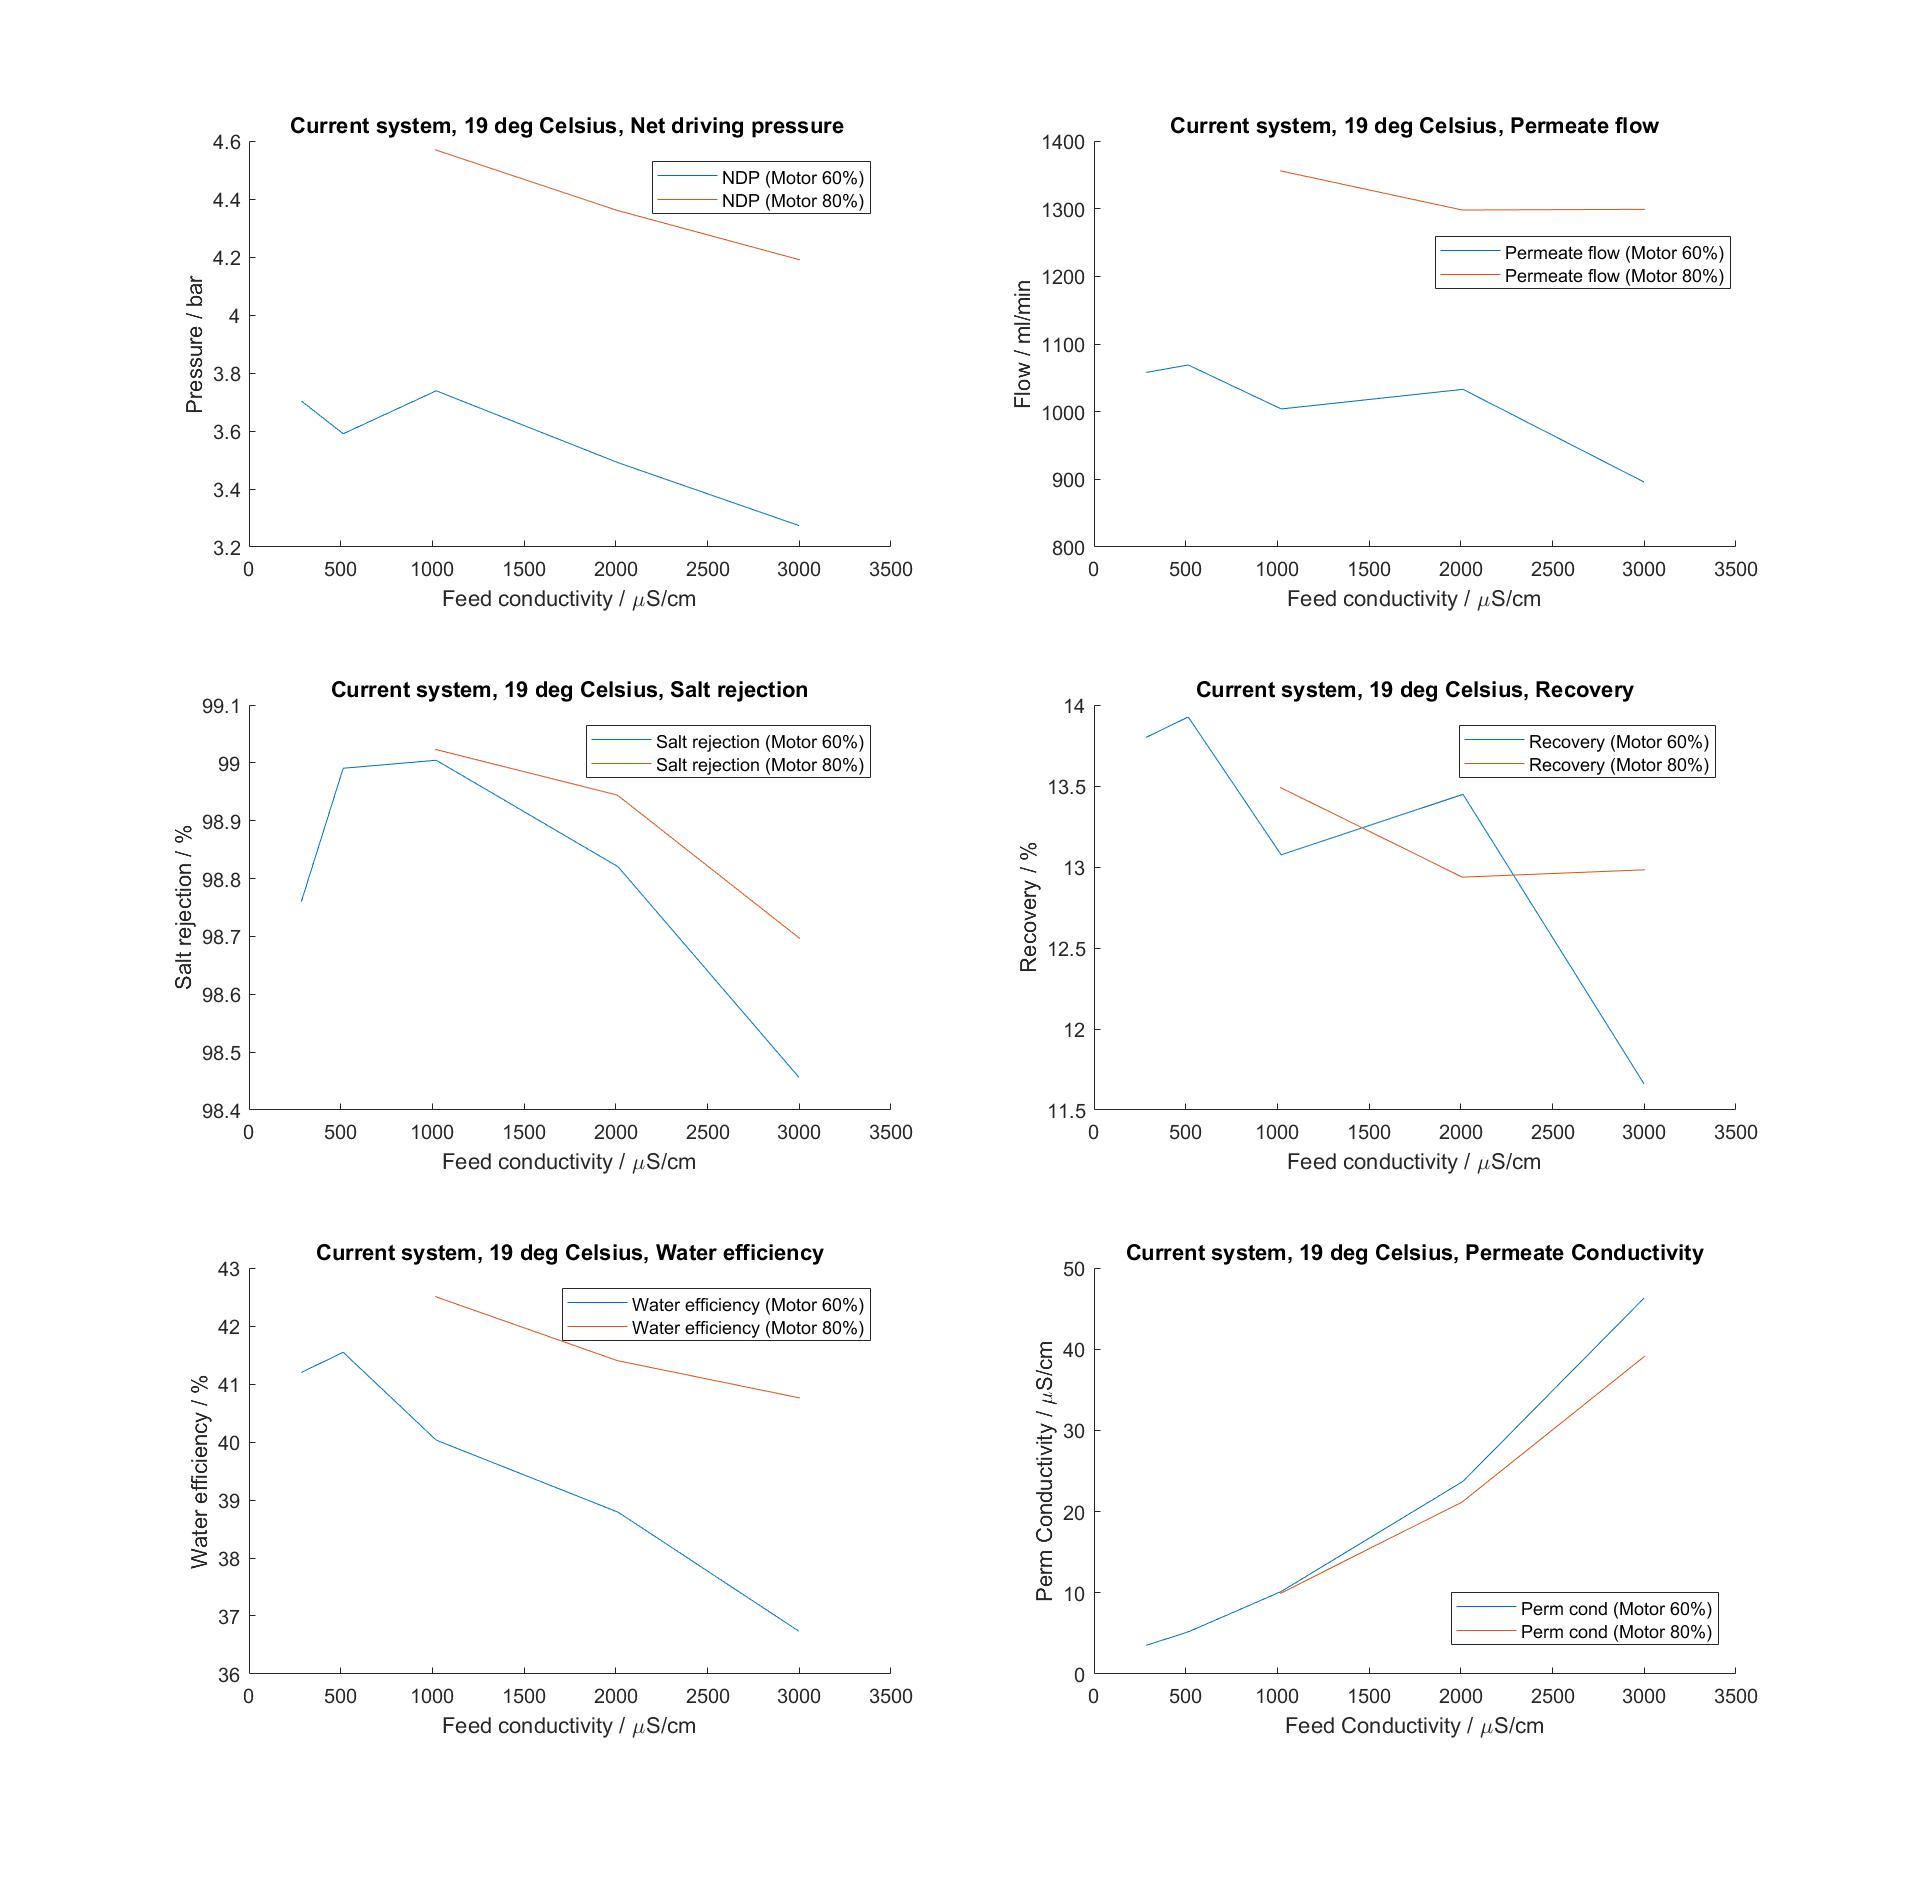
\includegraphics[width=1.1\textwidth]{Key20}
    \caption{Connections Pressure sensors}
    \label{fig:PressConn}
\end{figure}

\newpage
The second test was carried out by setting the heater bath to 30 degrees celsius and sweeping the conductivity from 280 uS/cm to 3000 uS/cm. To save time, all steady states were investigated in the same test.  

\begin{figure}[H]
    \centering
    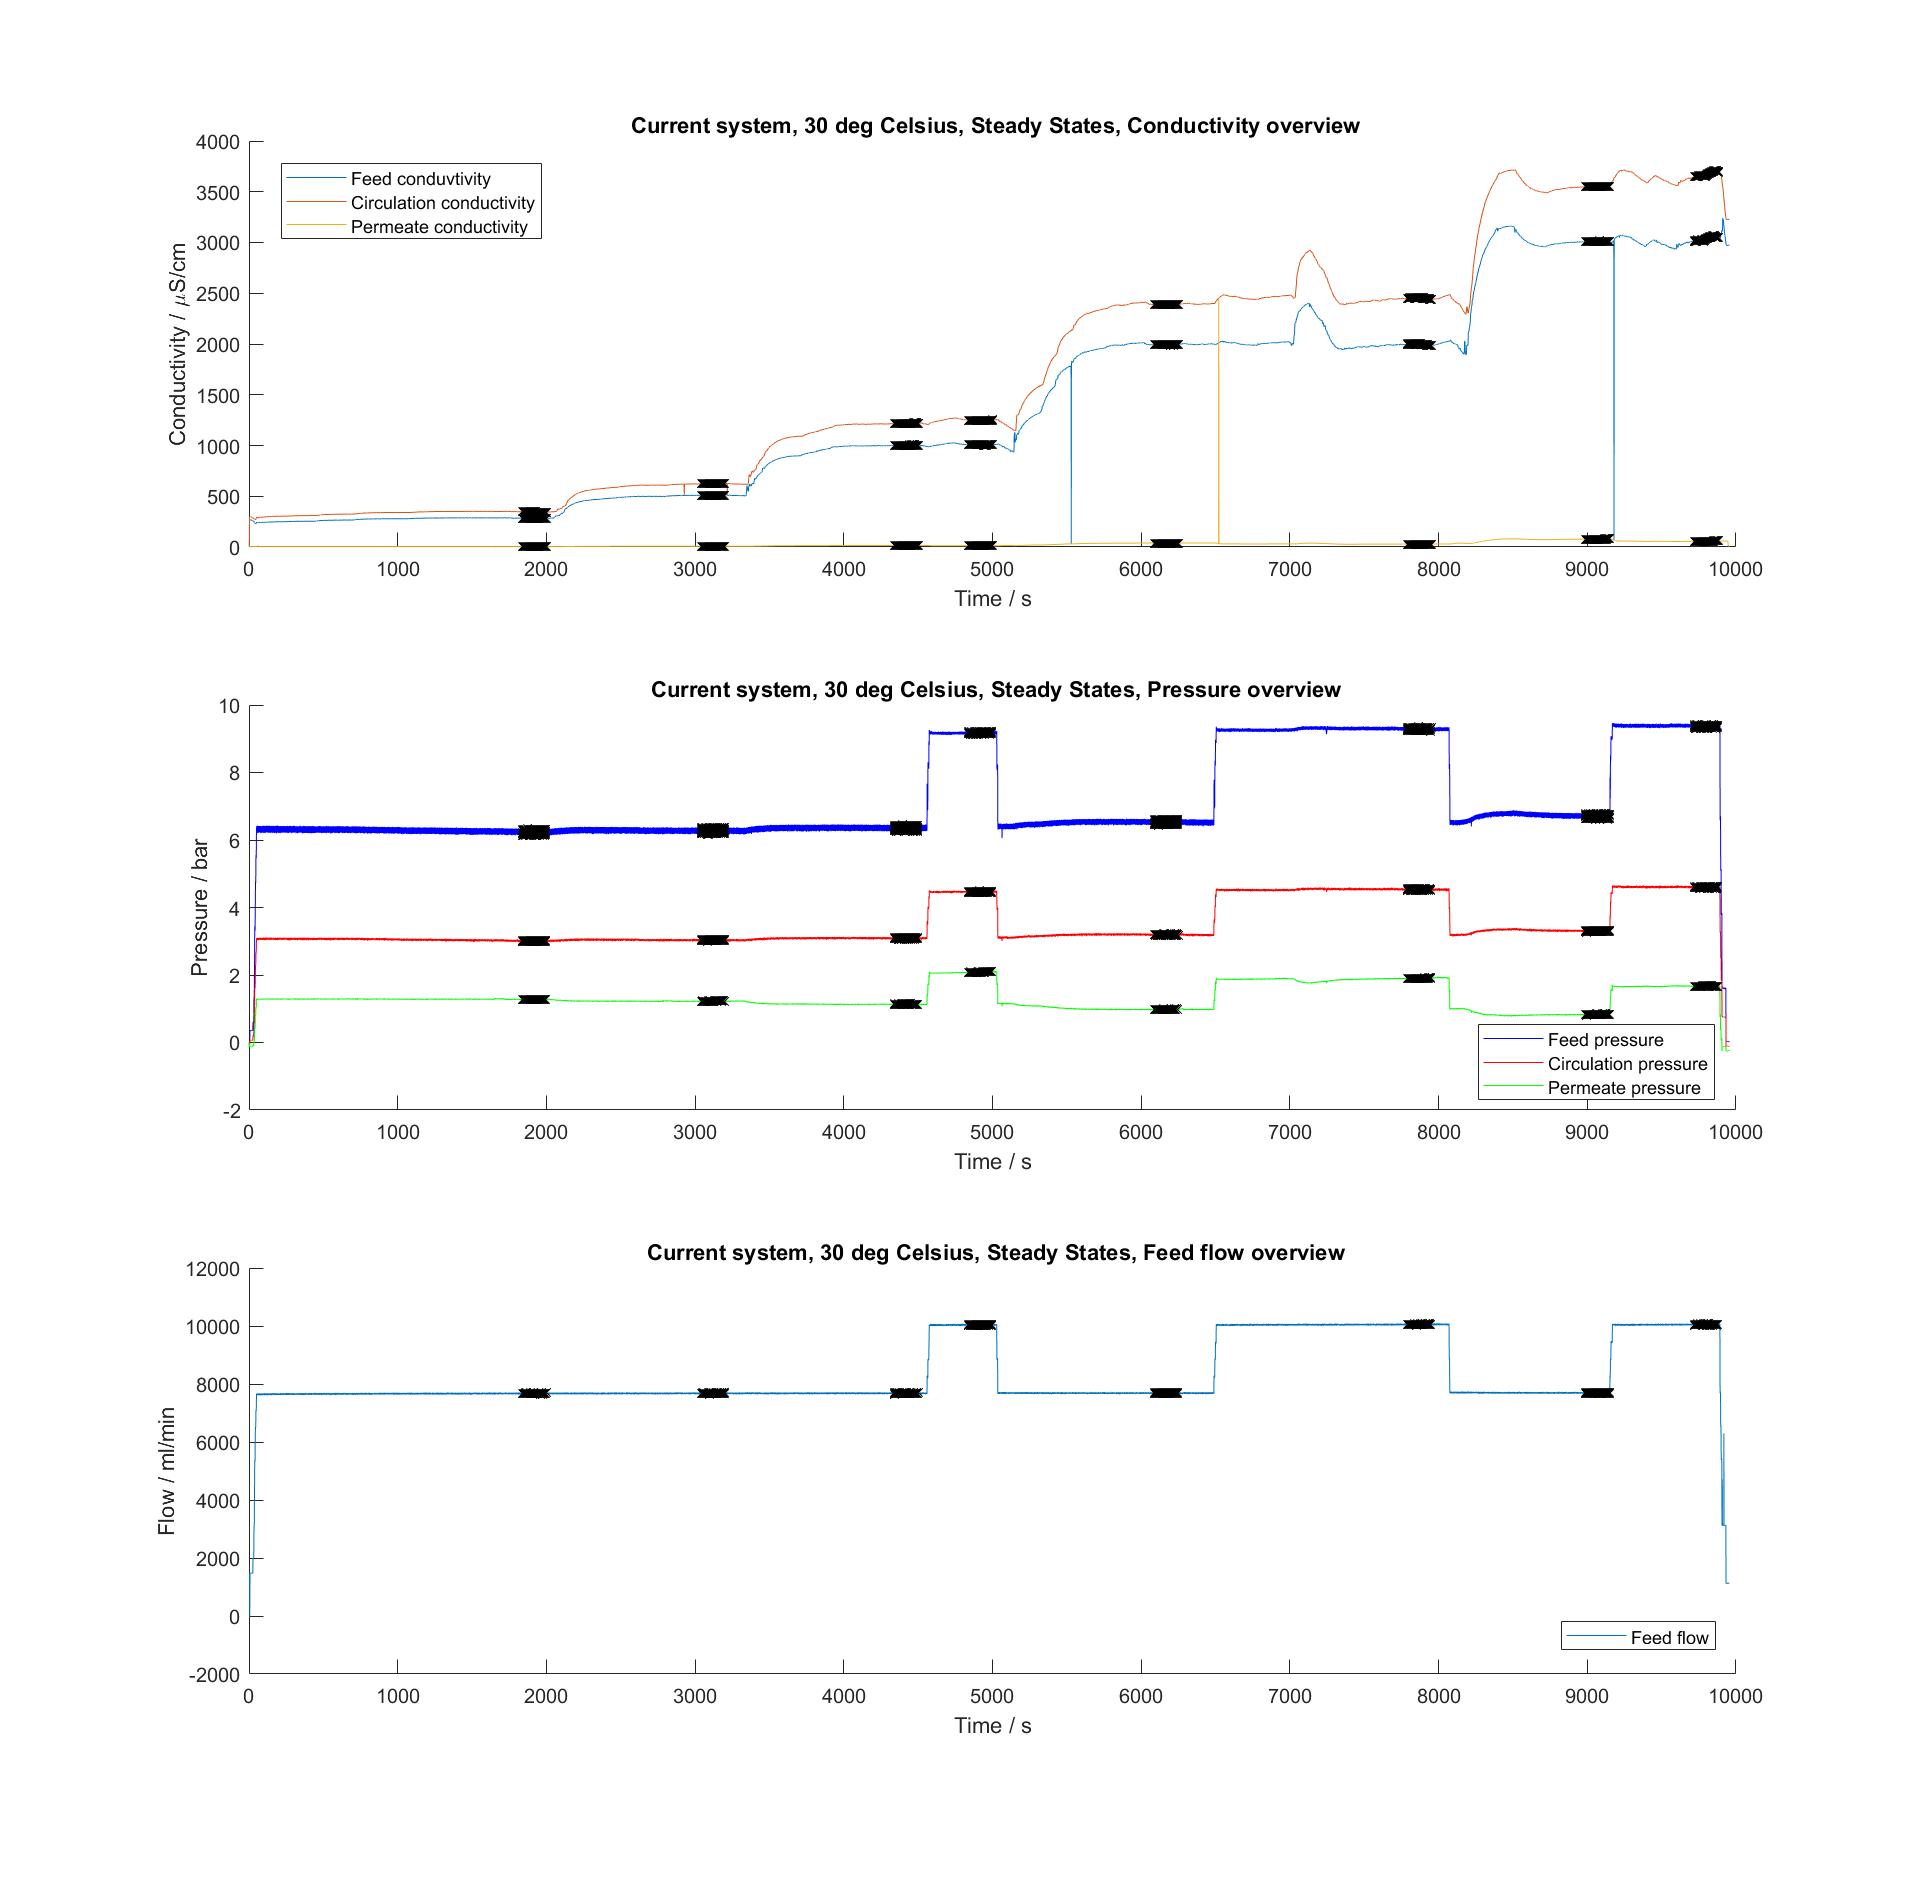
\includegraphics[width=1.1\textwidth]{overview30}
    \caption{Test 2, Current system, 30 degrees celsius. Steady states 1.1, 1.2, 1.3, 1.4 1.5, 1.6, 1.7 and 1.8}
    \label{fig:PressConn}
\end{figure}

\newpage

The important parameters were investigated for every steady state.

\begin{figure}[H]
    \centering
    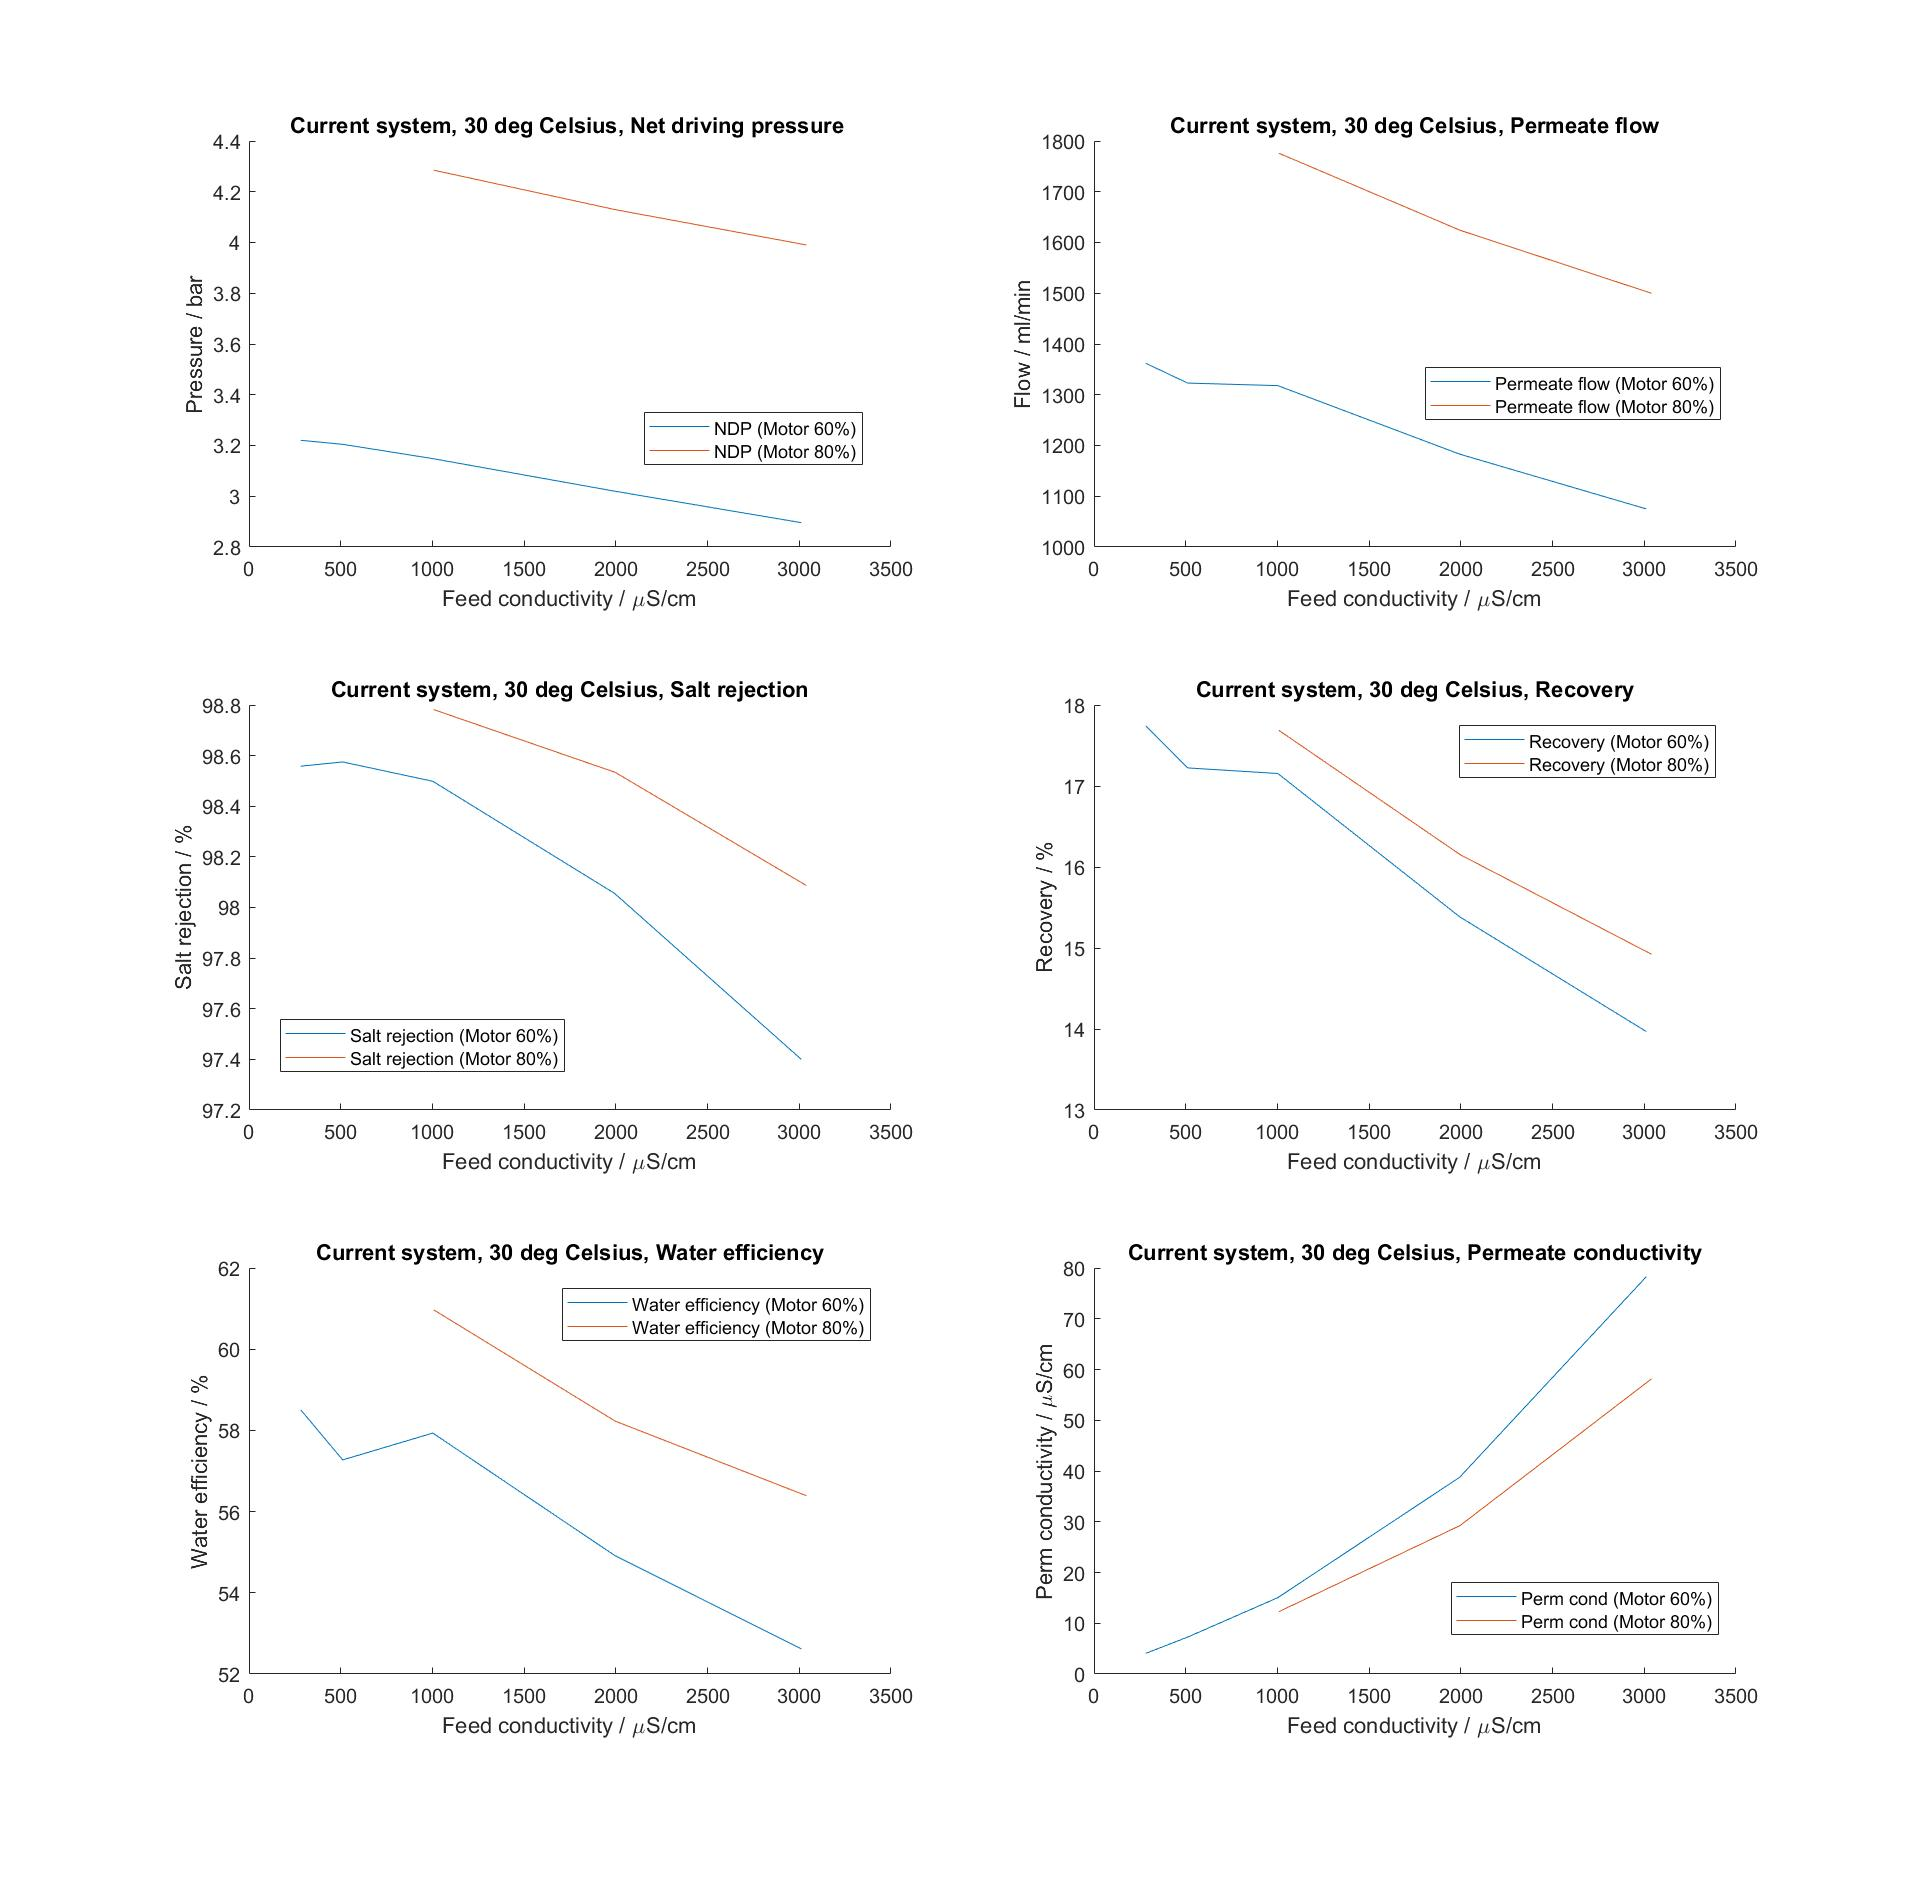
\includegraphics[width=1.1\textwidth]{Key30}
    \caption{Connections Pressure sensors}
    \label{fig:PressConn}
\end{figure}

\newpage

The heating bath was set to 40 degrees celsius before running test 3.

\begin{figure}[H]
    \centering
    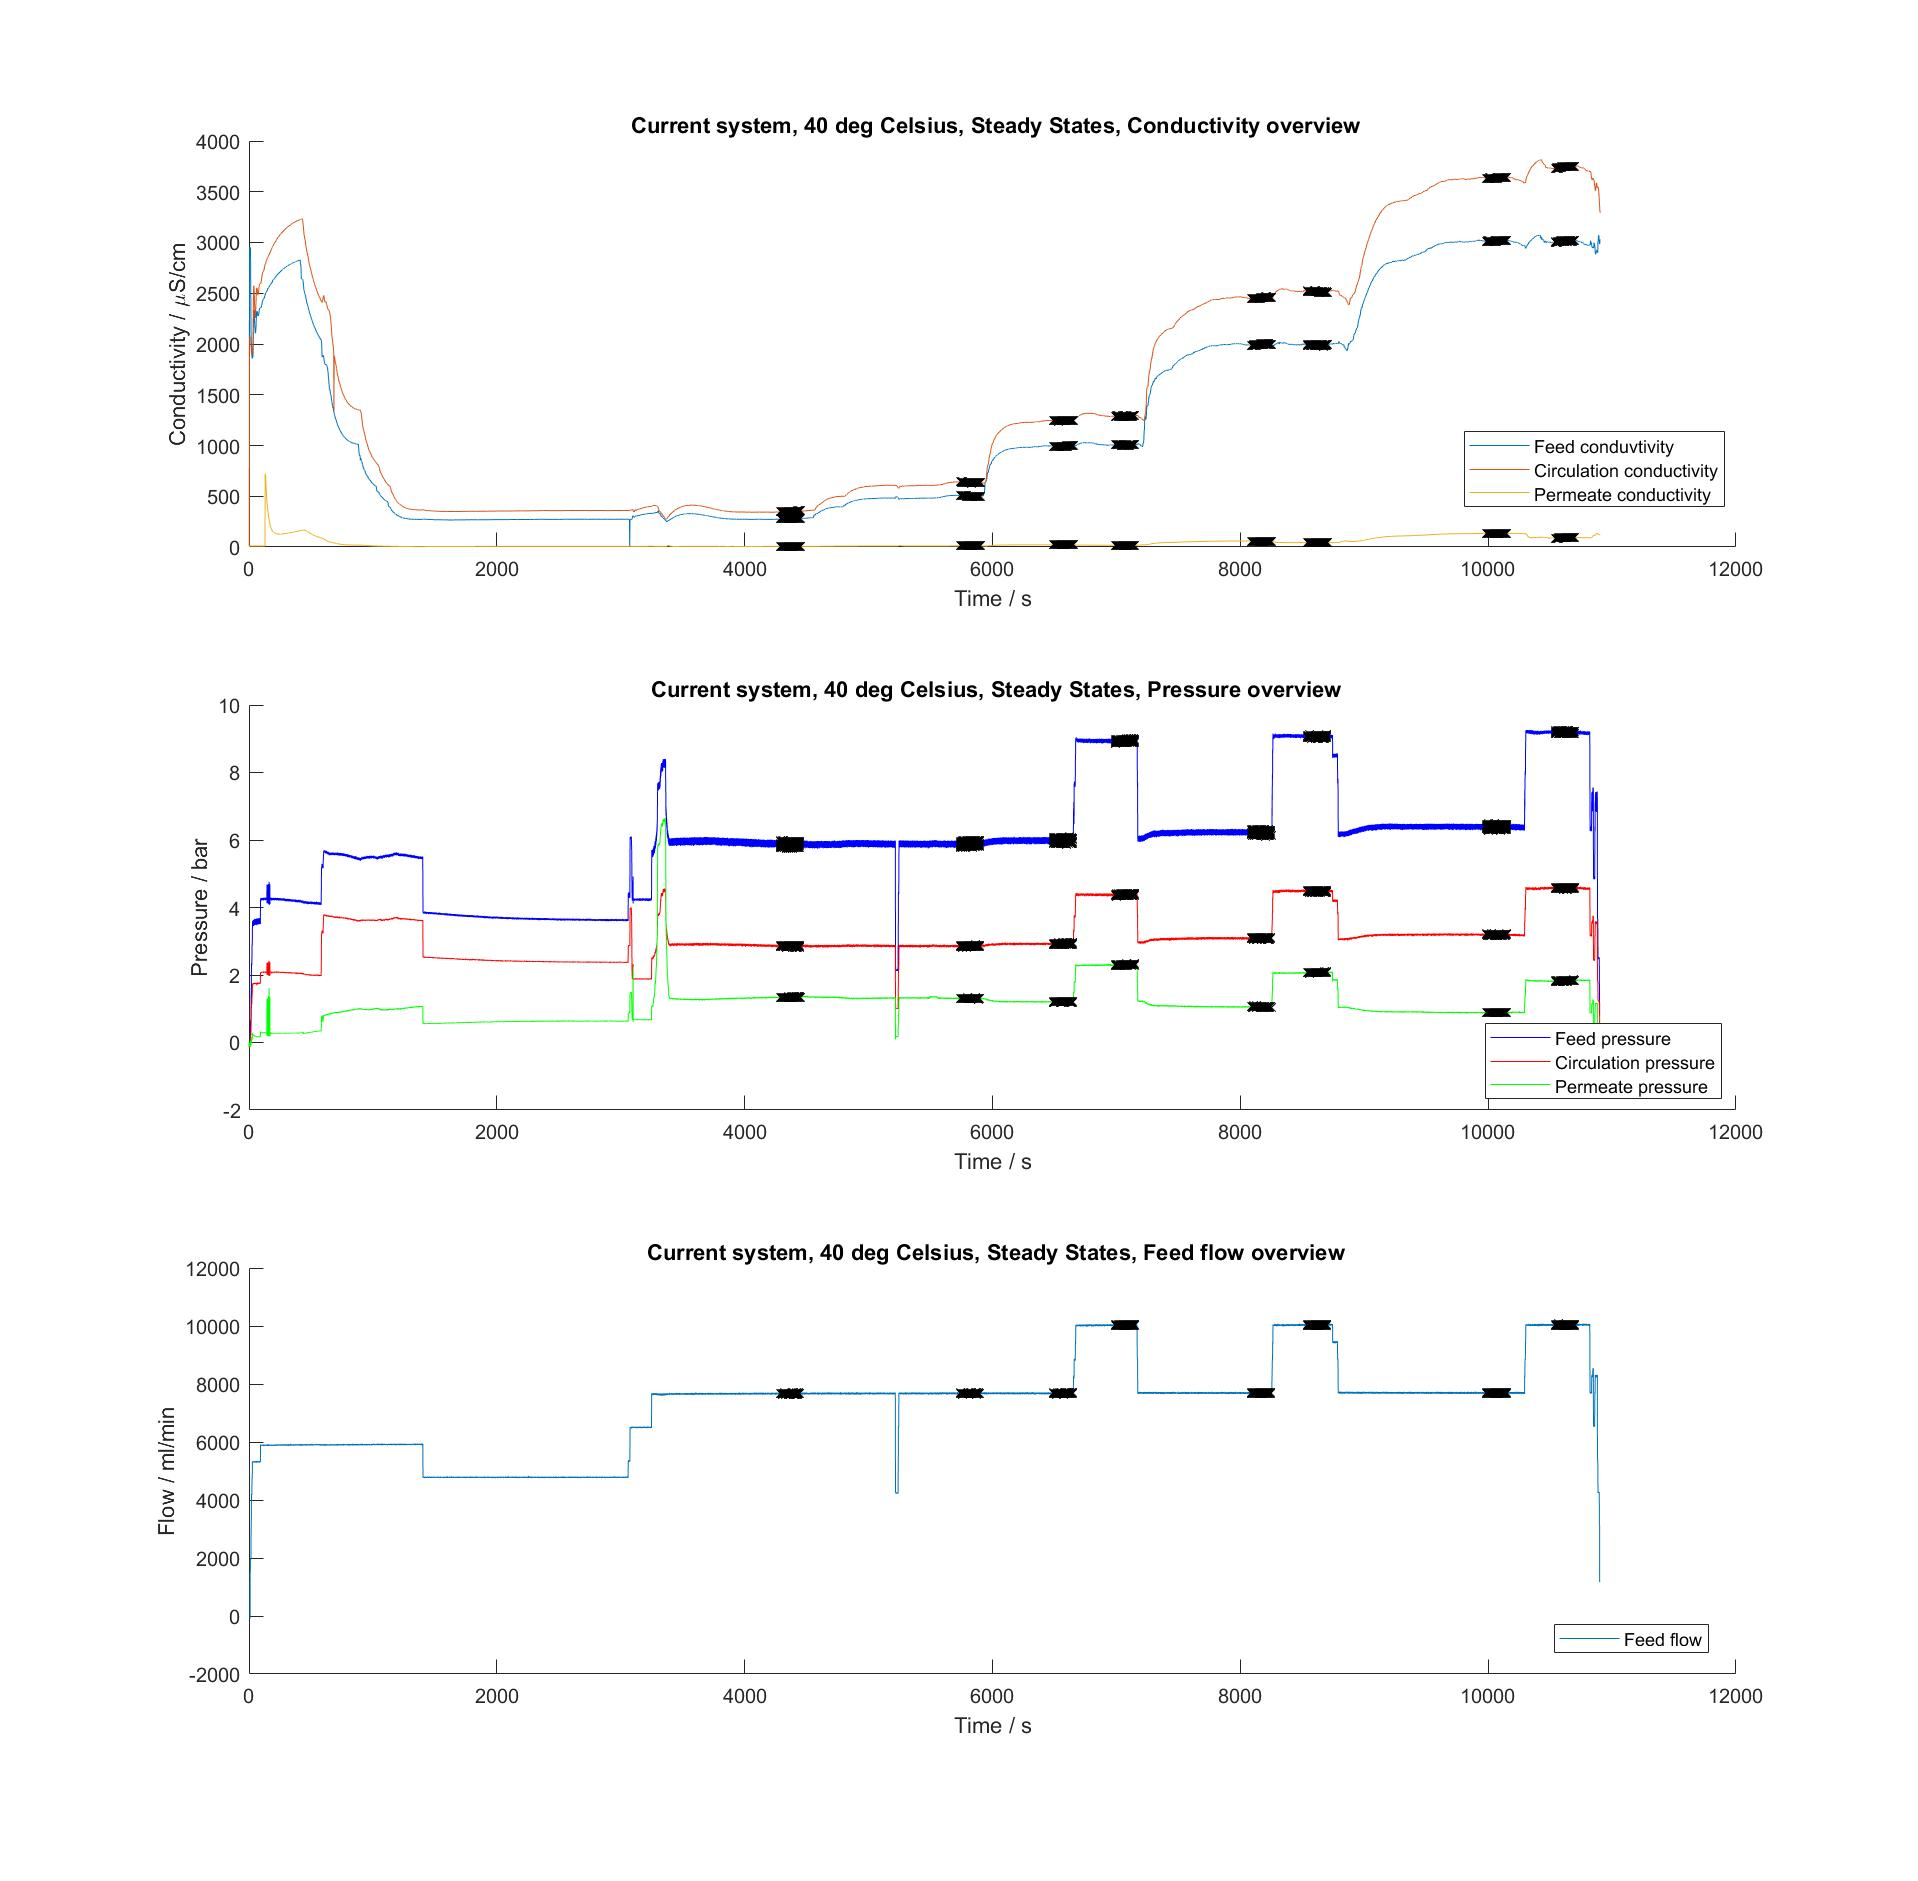
\includegraphics[width=1.1\textwidth]{overview40}
    \caption{Connections Pressure sensors}
    \label{fig:PressConn}
\end{figure}

\newpage

The important parameters were investigated for every steady state.
\begin{figure}[H]
    \centering
    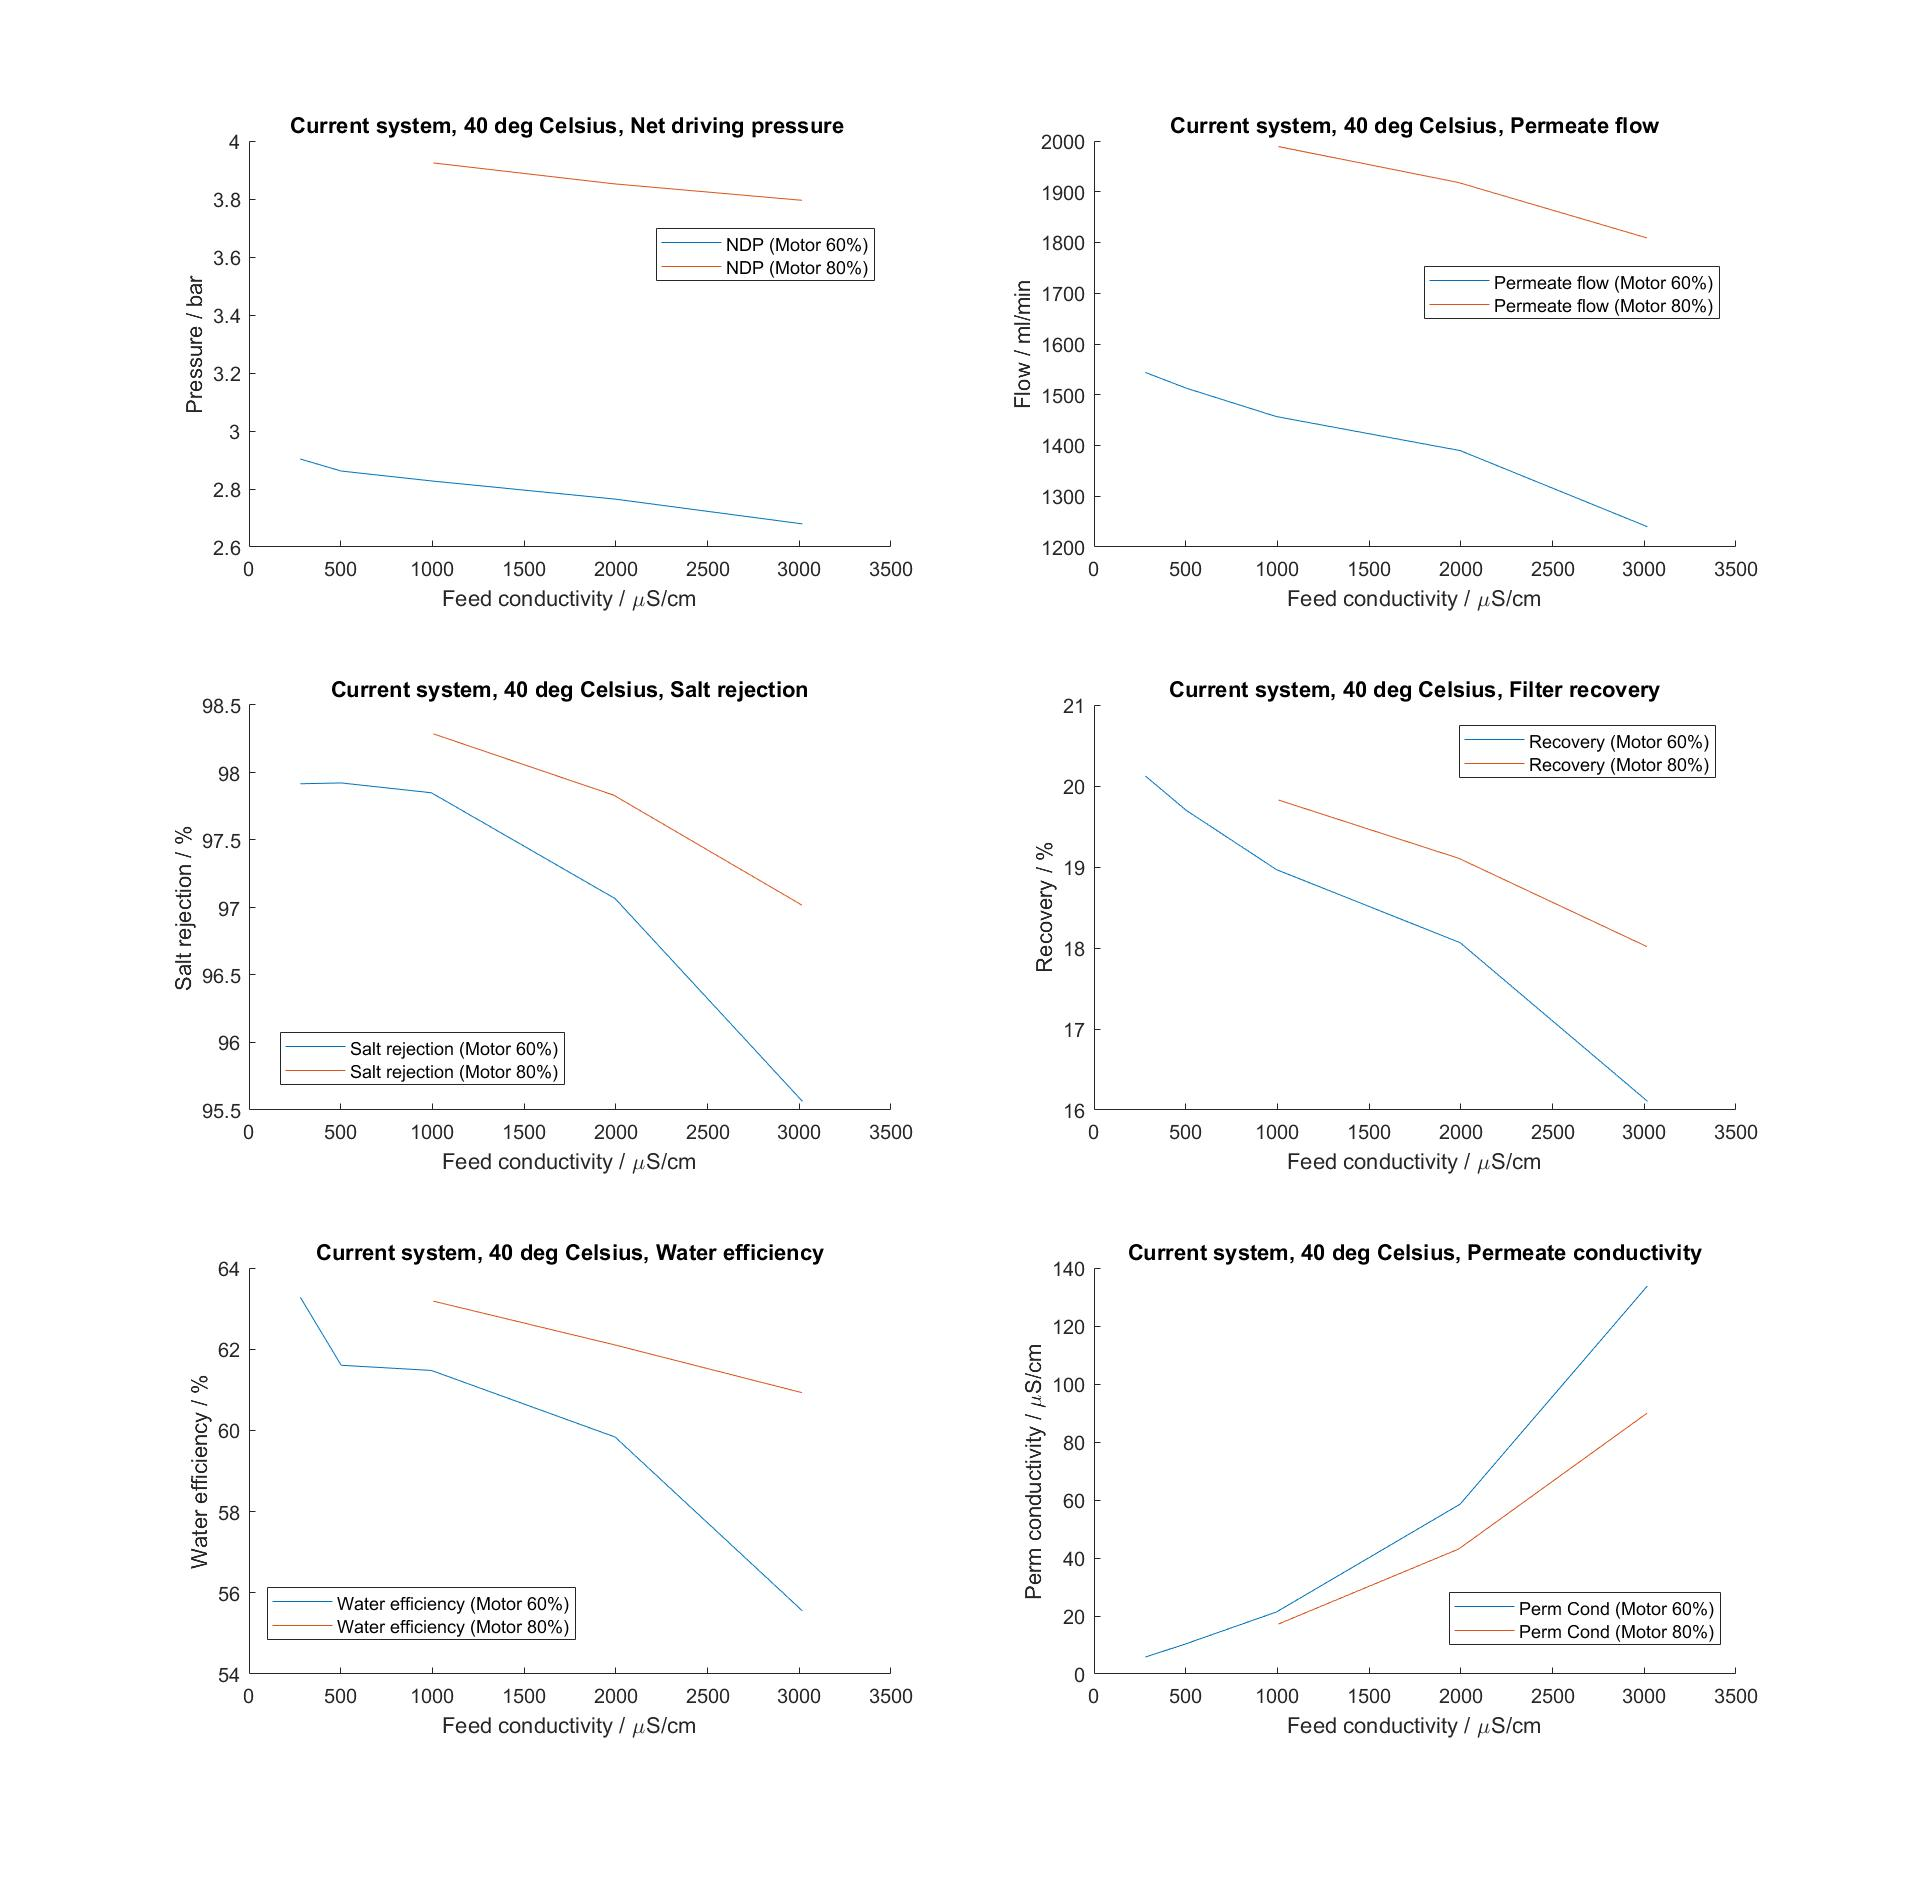
\includegraphics[width=1.1\textwidth]{Key40}
    \caption{Connections Pressure sensors}
    \label{fig:PressConn}
\end{figure}

By plotting the data from the three tests it was possible to generate graphs that could visualize how temperature, conductivity and feed pressure affected the membrane.

\begin{figure}[H]
    \centering
    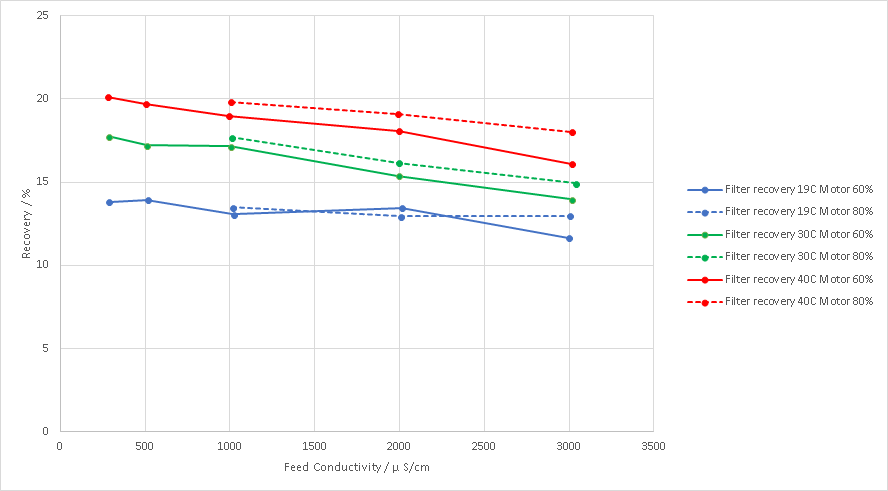
\includegraphics[width=1.1\textwidth]{Recovery}
    \caption{Connections Pressure sensors}
    \label{fig:PressConn}
\end{figure}

\begin{figure}[H]
    \centering
    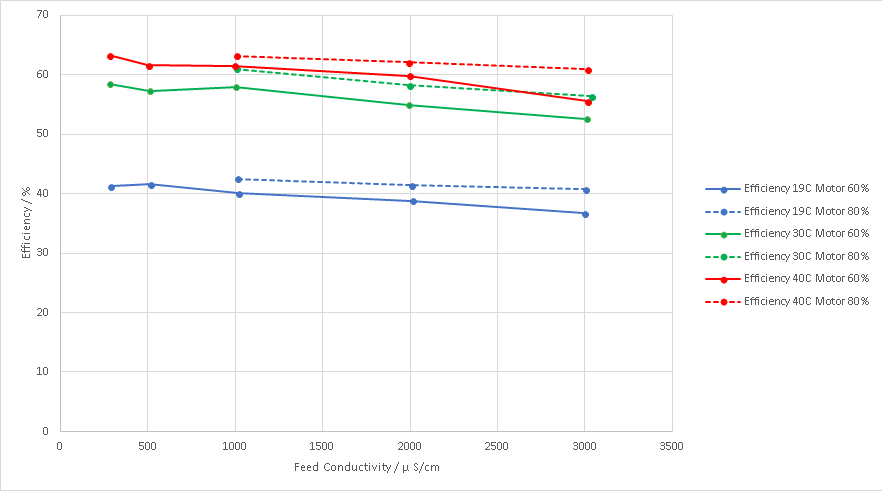
\includegraphics[width=1.1\textwidth]{Efficiency}
    \caption{Connections Pressure sensors}
    \label{fig:PressConn}
\end{figure}

\begin{figure}[H]
    \centering
    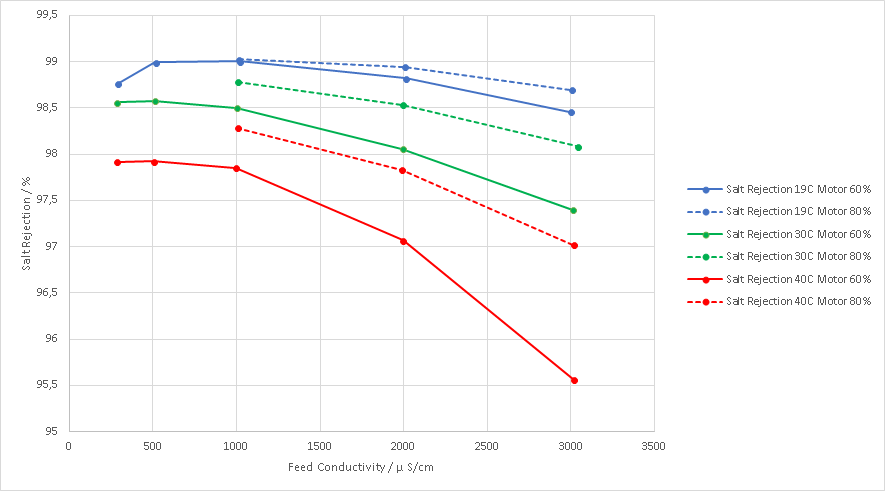
\includegraphics[width=1.1\textwidth]{SaltRejection}
    \caption{Connections Pressure sensors}
    \label{fig:PressConn}
\end{figure}

\begin{figure}[H]
    \centering
    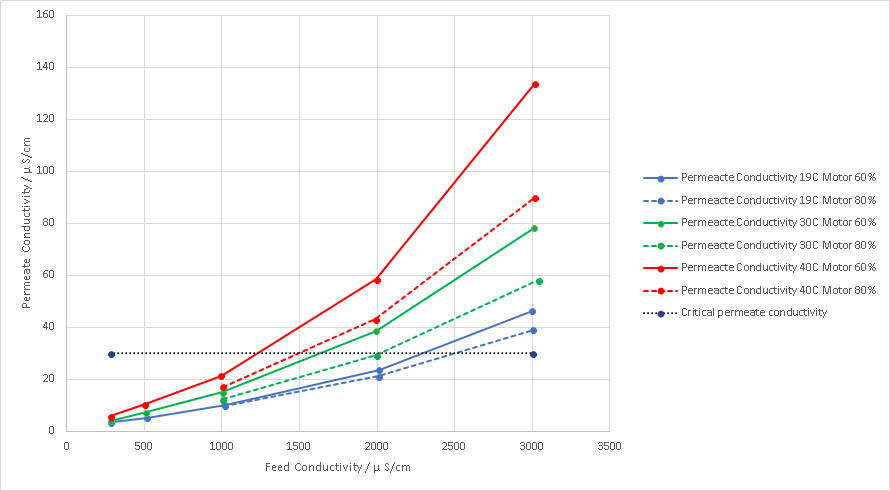
\includegraphics[width=1.1\textwidth]{PermCond}
    \caption{Connections Pressure sensors}
    \label{fig:PressConn}
\end{figure}

\begin{figure}[H]
    \centering
    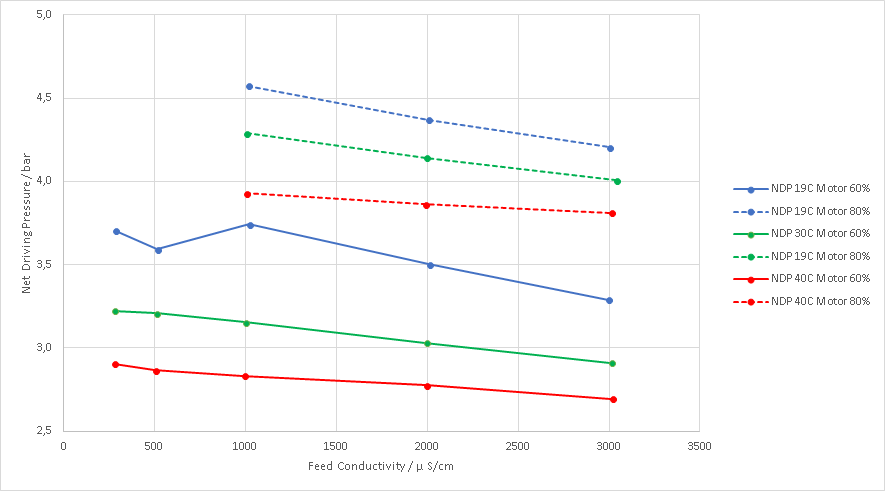
\includegraphics[width=1.1\textwidth]{NDP}
    \caption{Connections Pressure sensors}
    \label{fig:PressConn}
\end{figure}

\begin{figure}[H]
    \centering
    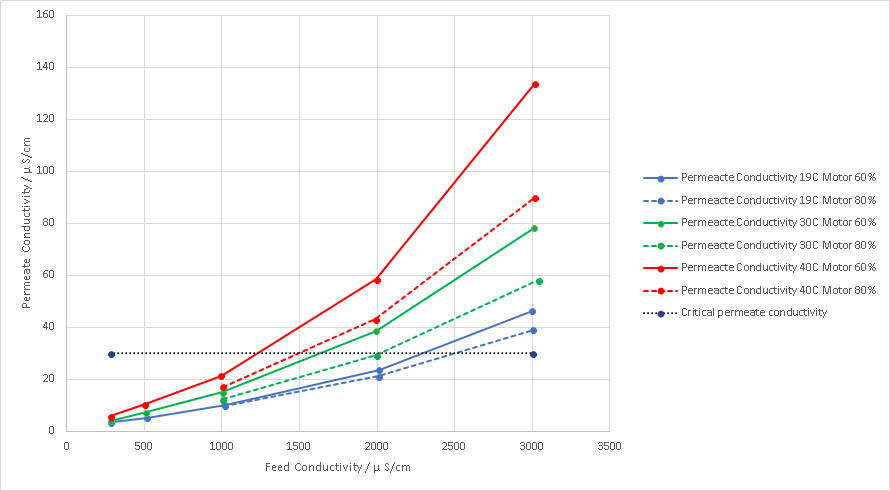
\includegraphics[width=1.1\textwidth]{PermCond}
    \caption{Connections Pressure sensors}
    \label{fig:PressConn}
\end{figure}





\subsection{System 2}

Test: increaed feed pressure

21


\begin{figure}[H]
    \centering
    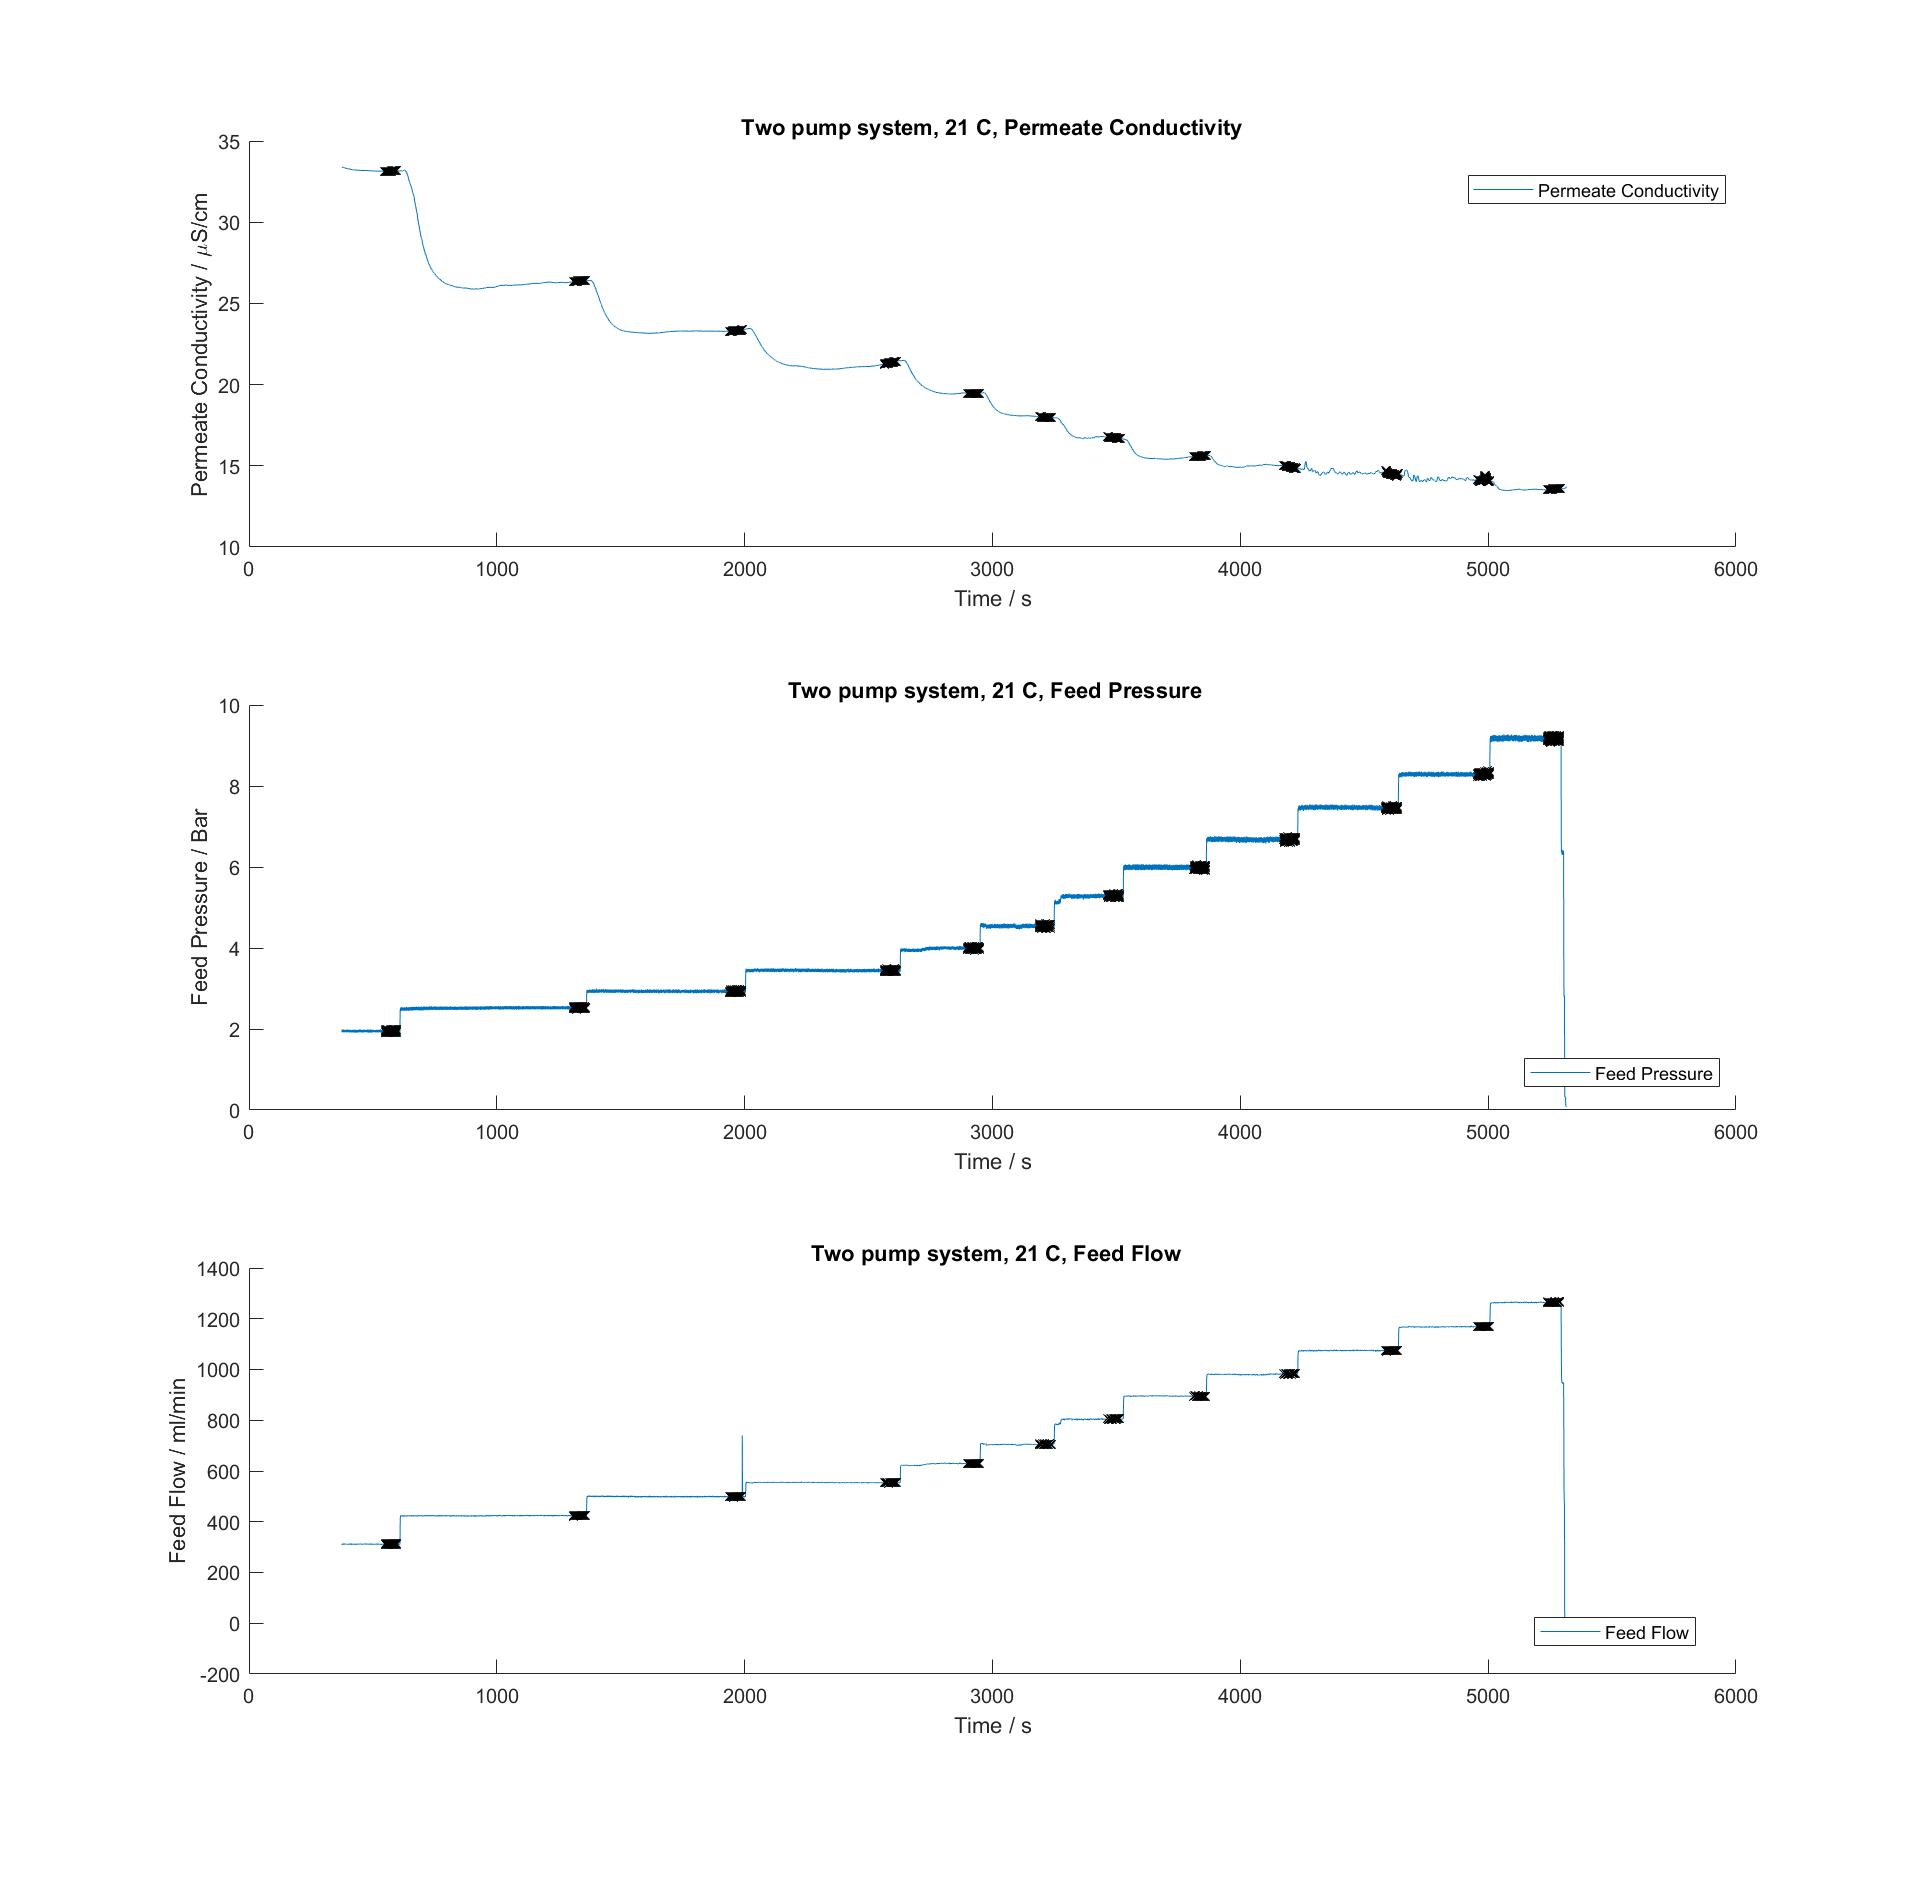
\includegraphics[width=1.1\textwidth]{FeedPumpIncrease21}
    \caption{Connections Pressure sensors}
    \label{fig:PressConn}
\end{figure}


\begin{figure}[H]
    \centering
    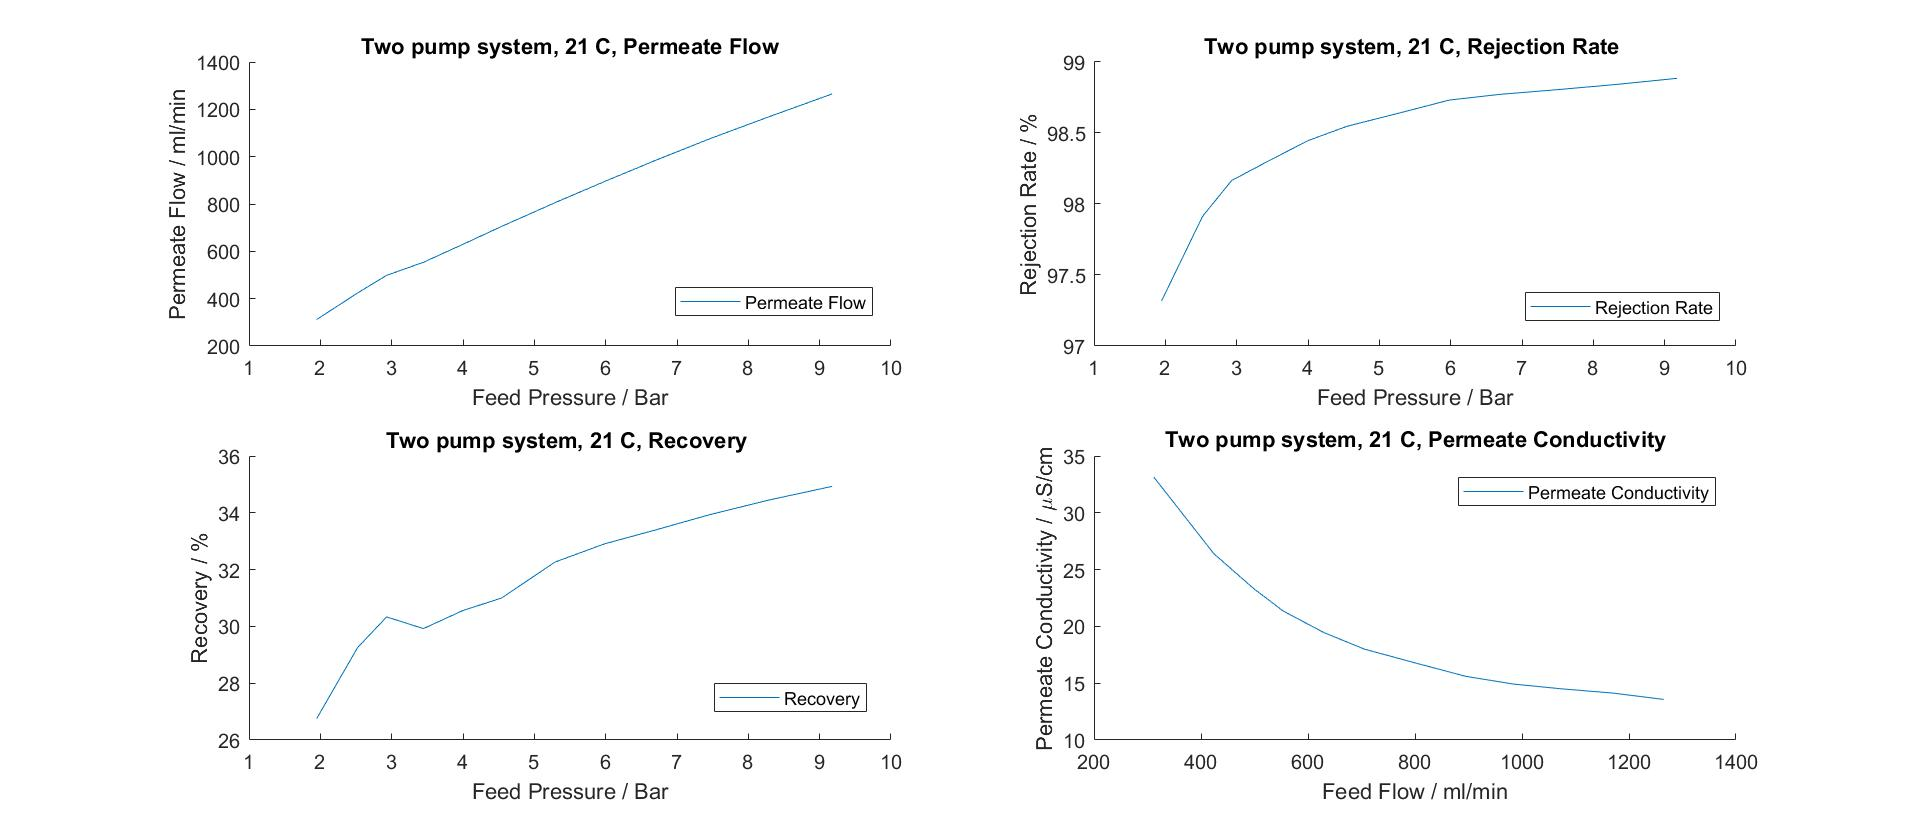
\includegraphics[width=1.1\textwidth]{FeedPumpIncrease21Key}
    \caption{Connections Pressure sensors}
    \label{fig:PressConn}
\end{figure}

30


\begin{figure}[H]
    \centering
    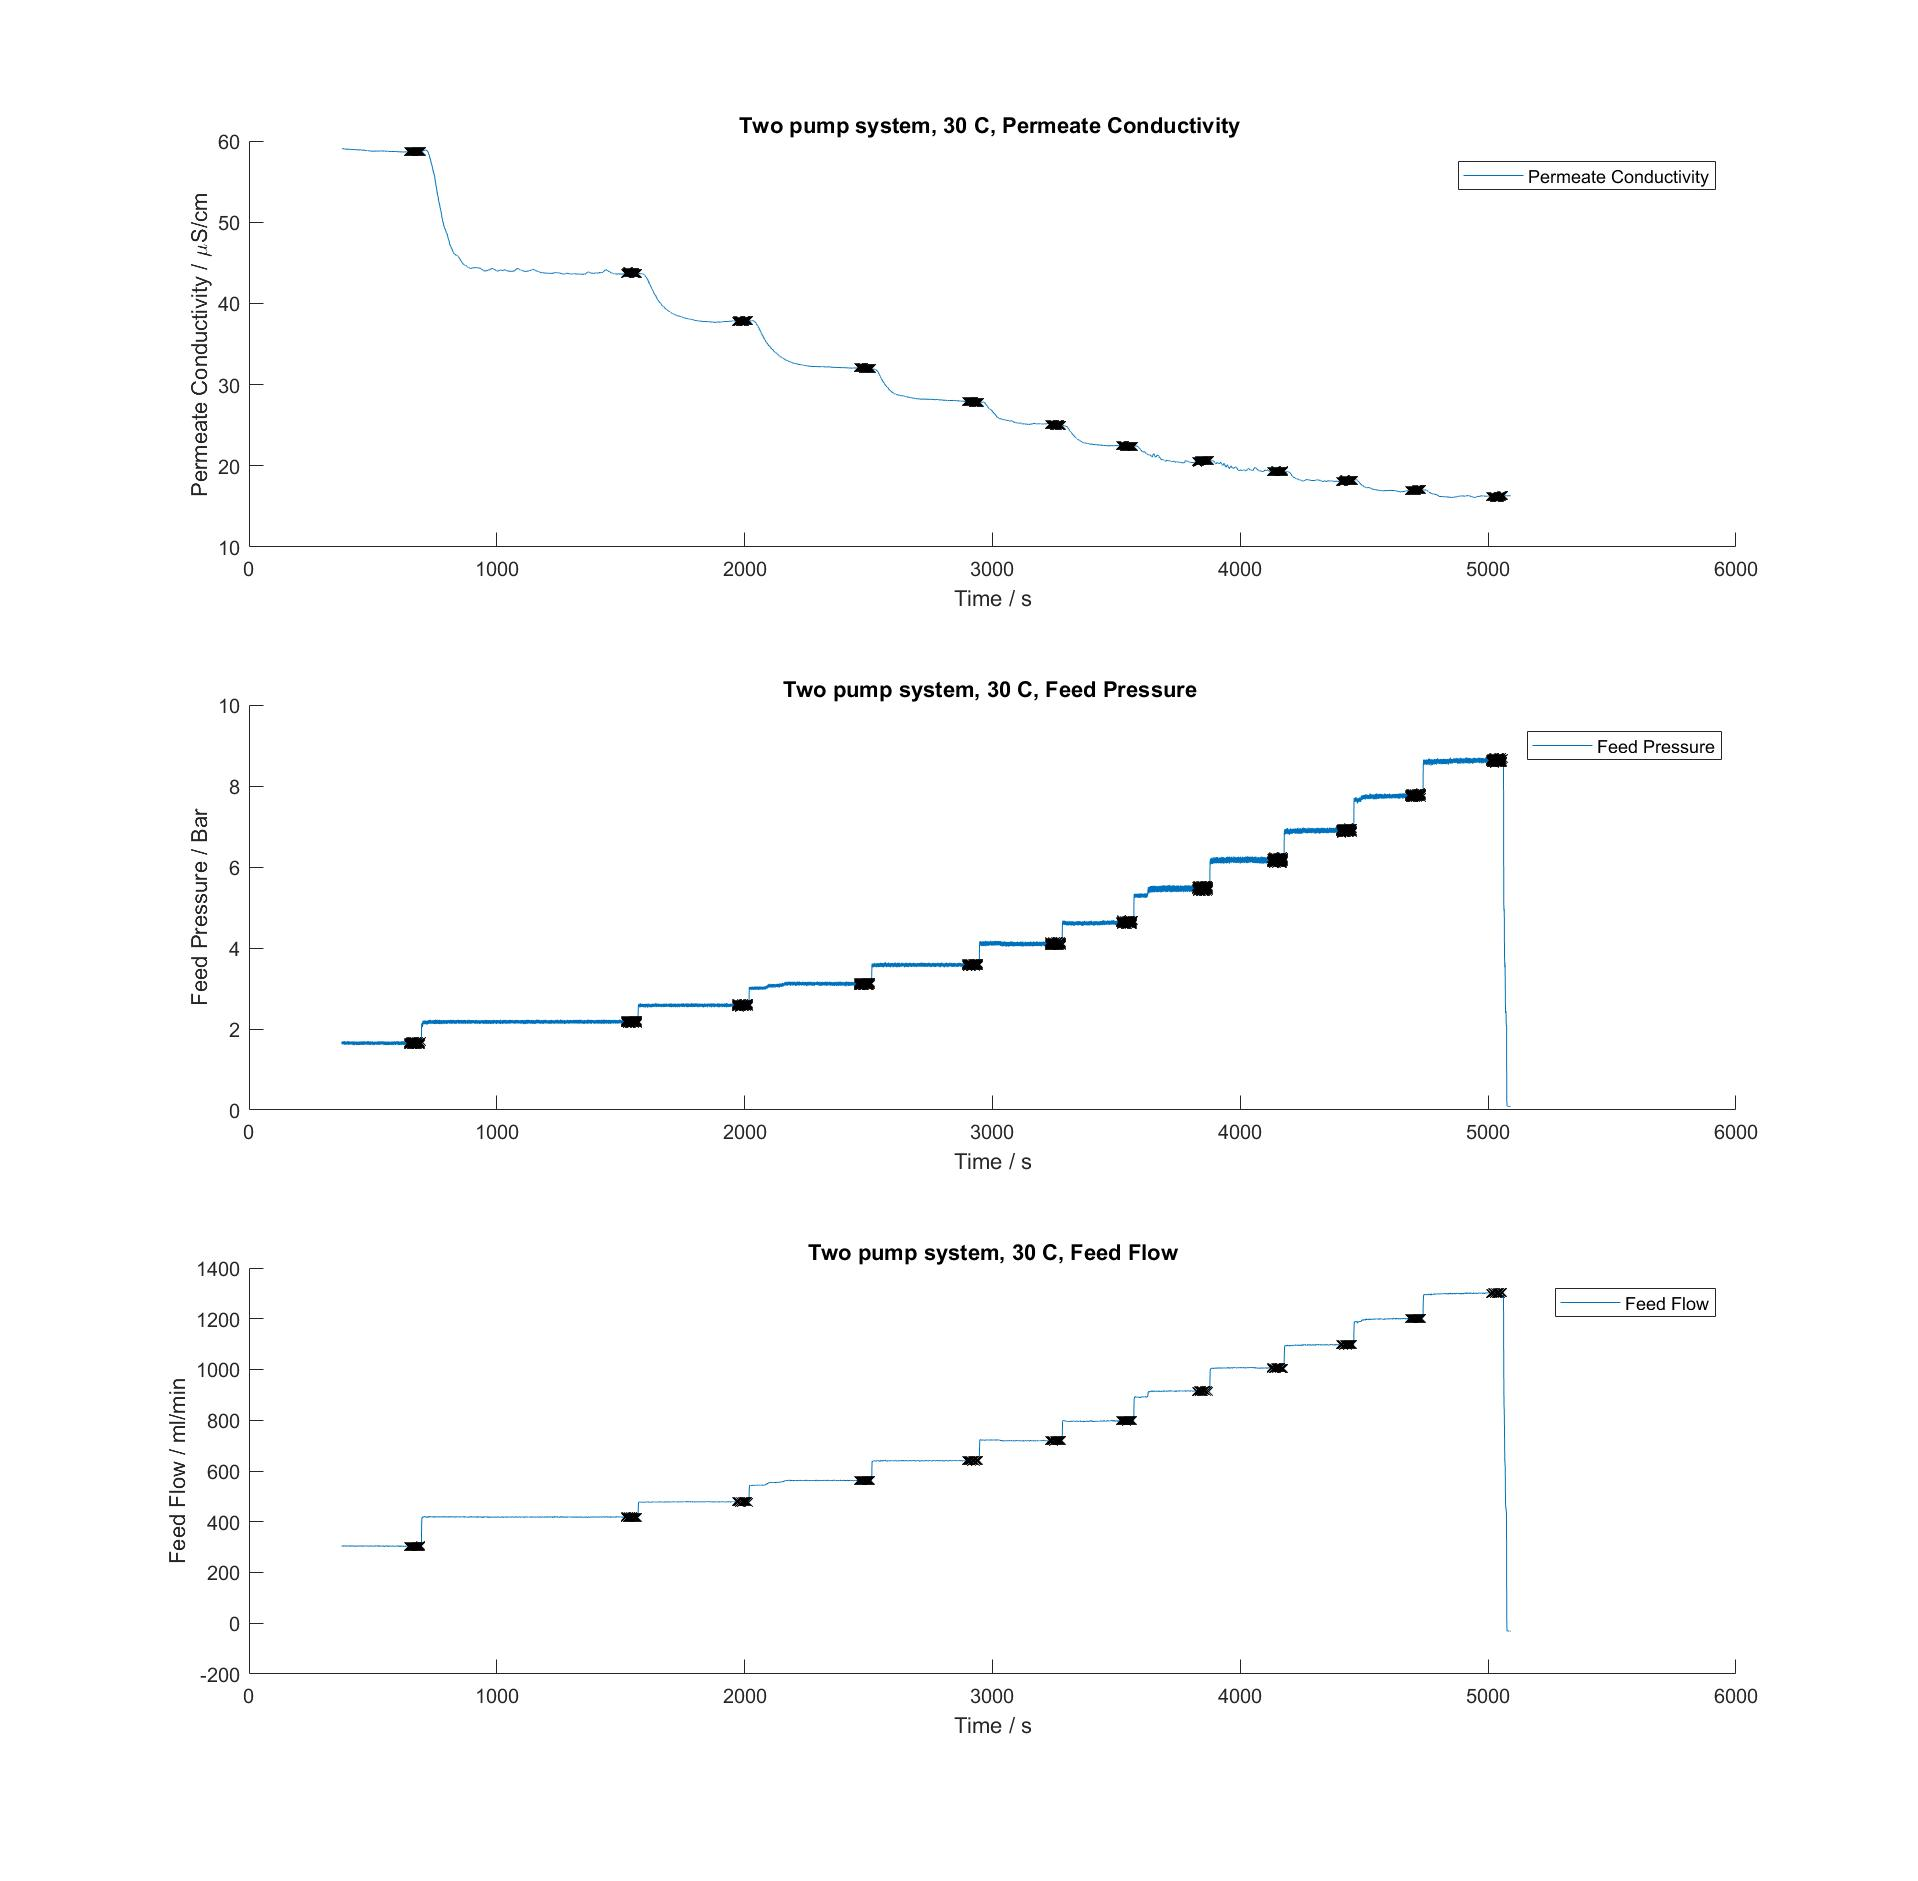
\includegraphics[width=1.1\textwidth]{FeedPumpIncrease30}
    \caption{Connections Pressure sensors}
    \label{fig:PressConn}
\end{figure}


\begin{figure}[H]
    \centering
    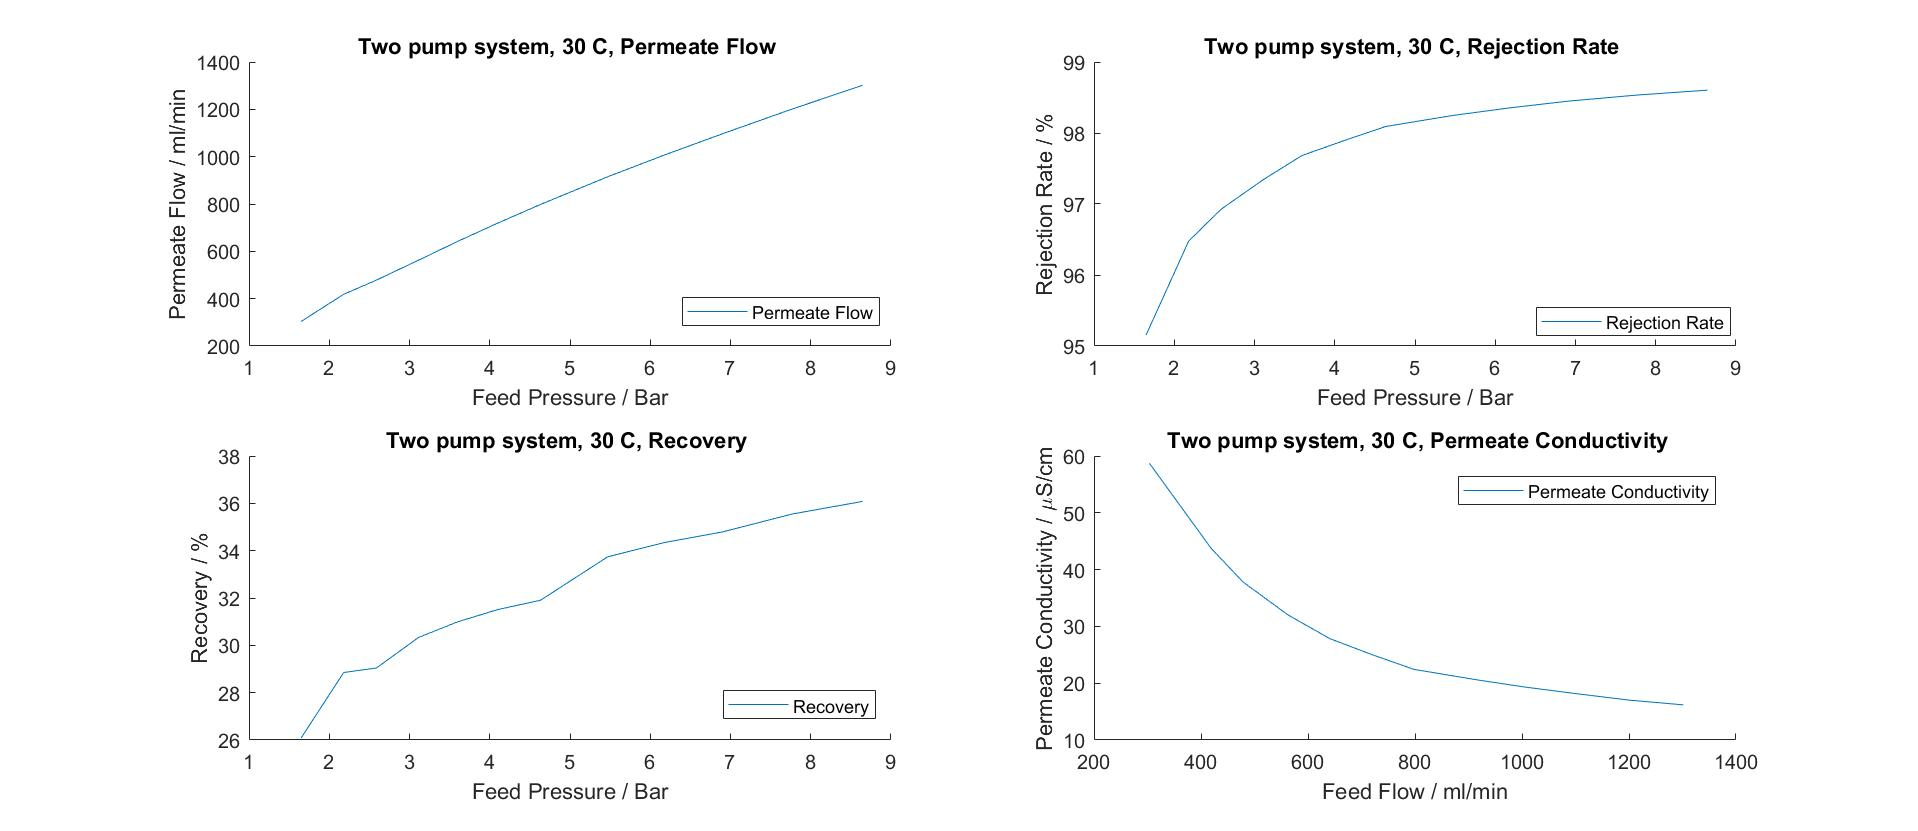
\includegraphics[width=1.1\textwidth]{FeedPumpIncrease30Key}
    \caption{Connections Pressure sensors}
    \label{fig:PressConn}
\end{figure}

40


\begin{figure}[H]
    \centering
    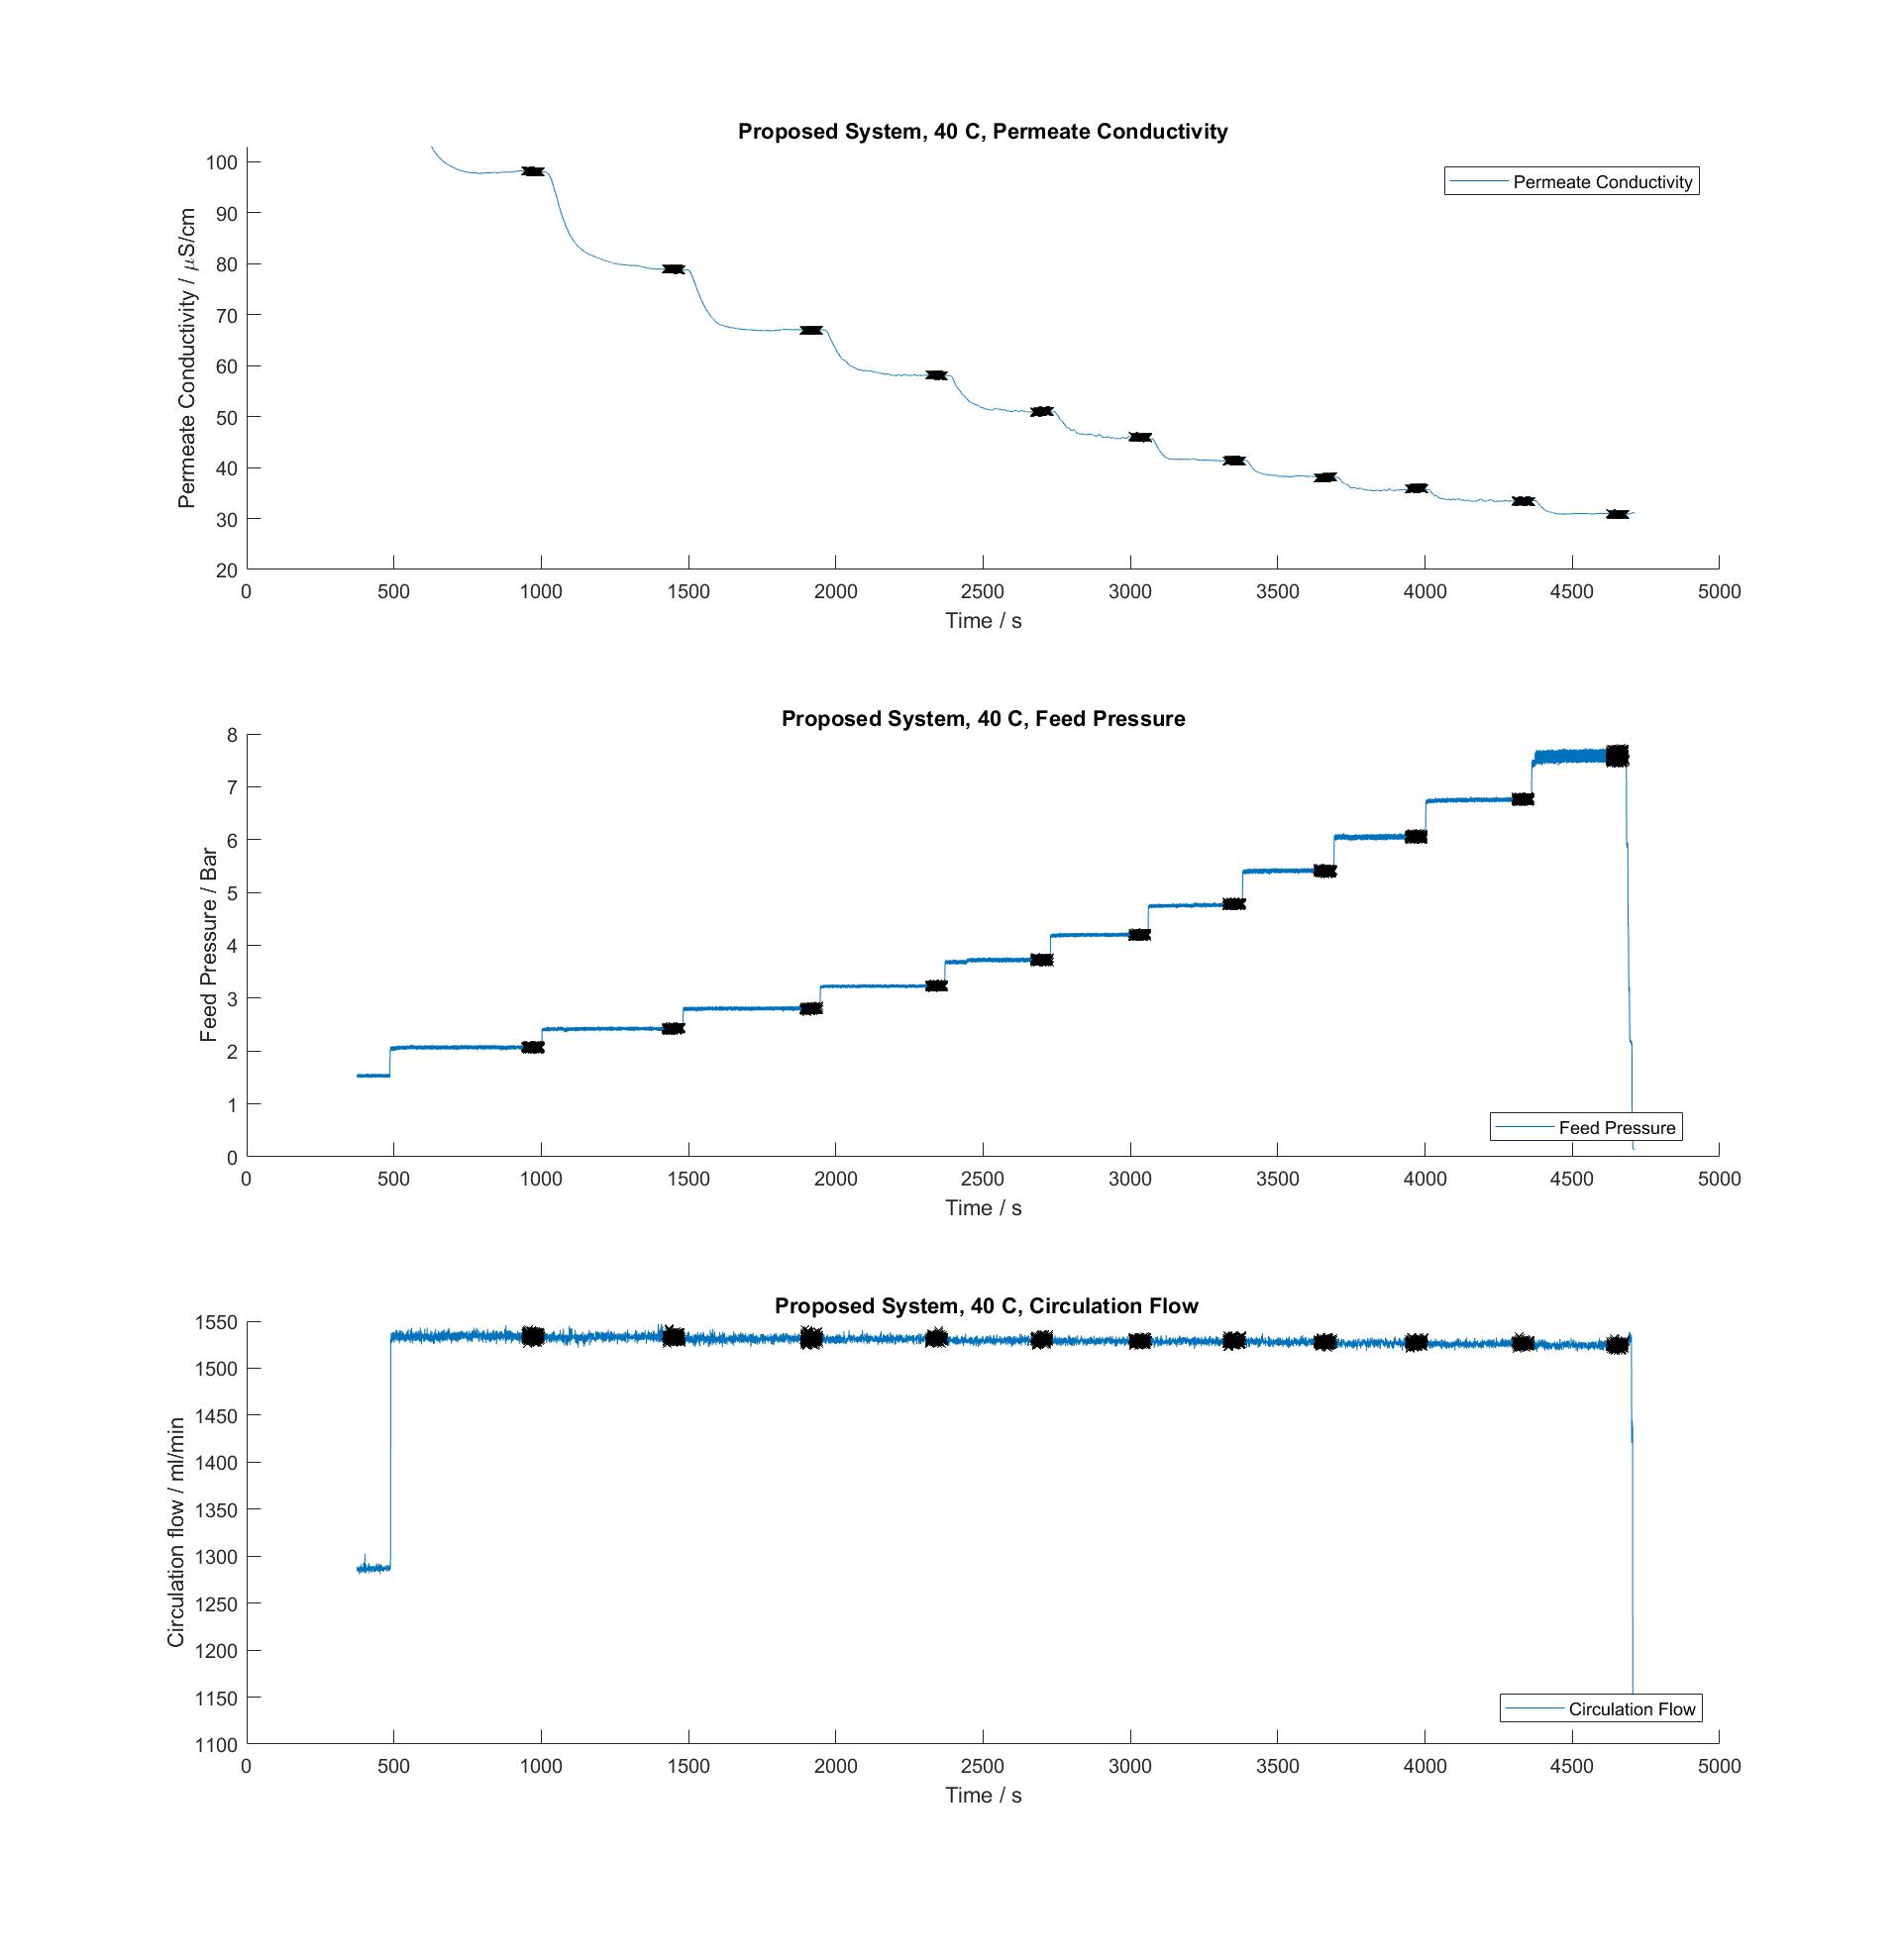
\includegraphics[width=1.1\textwidth]{FeedPumpIncrease40}
    \caption{Connections Pressure sensors}
    \label{fig:PressConn}
\end{figure}


\begin{figure}[H]
    \centering
    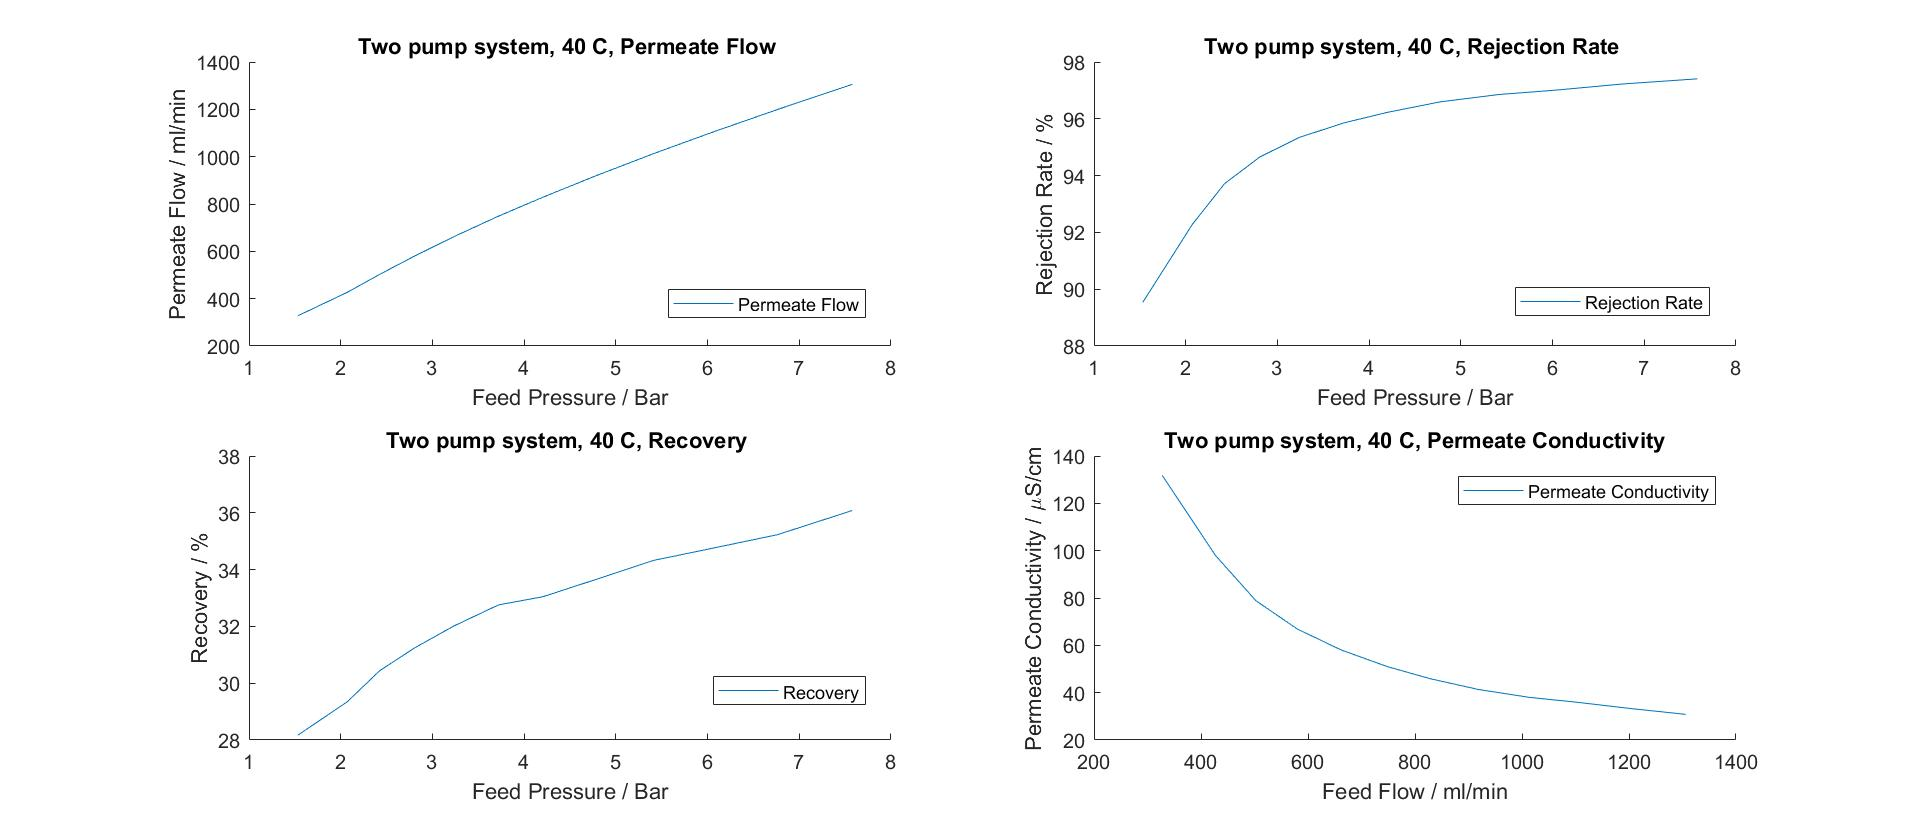
\includegraphics[width=1.1\textwidth]{FeedPumpIncrease40Key}
    \caption{Connections Pressure sensors}
    \label{fig:PressConn}
\end{figure}

Recovery Increase

\begin{figure}[H]
    \centering
    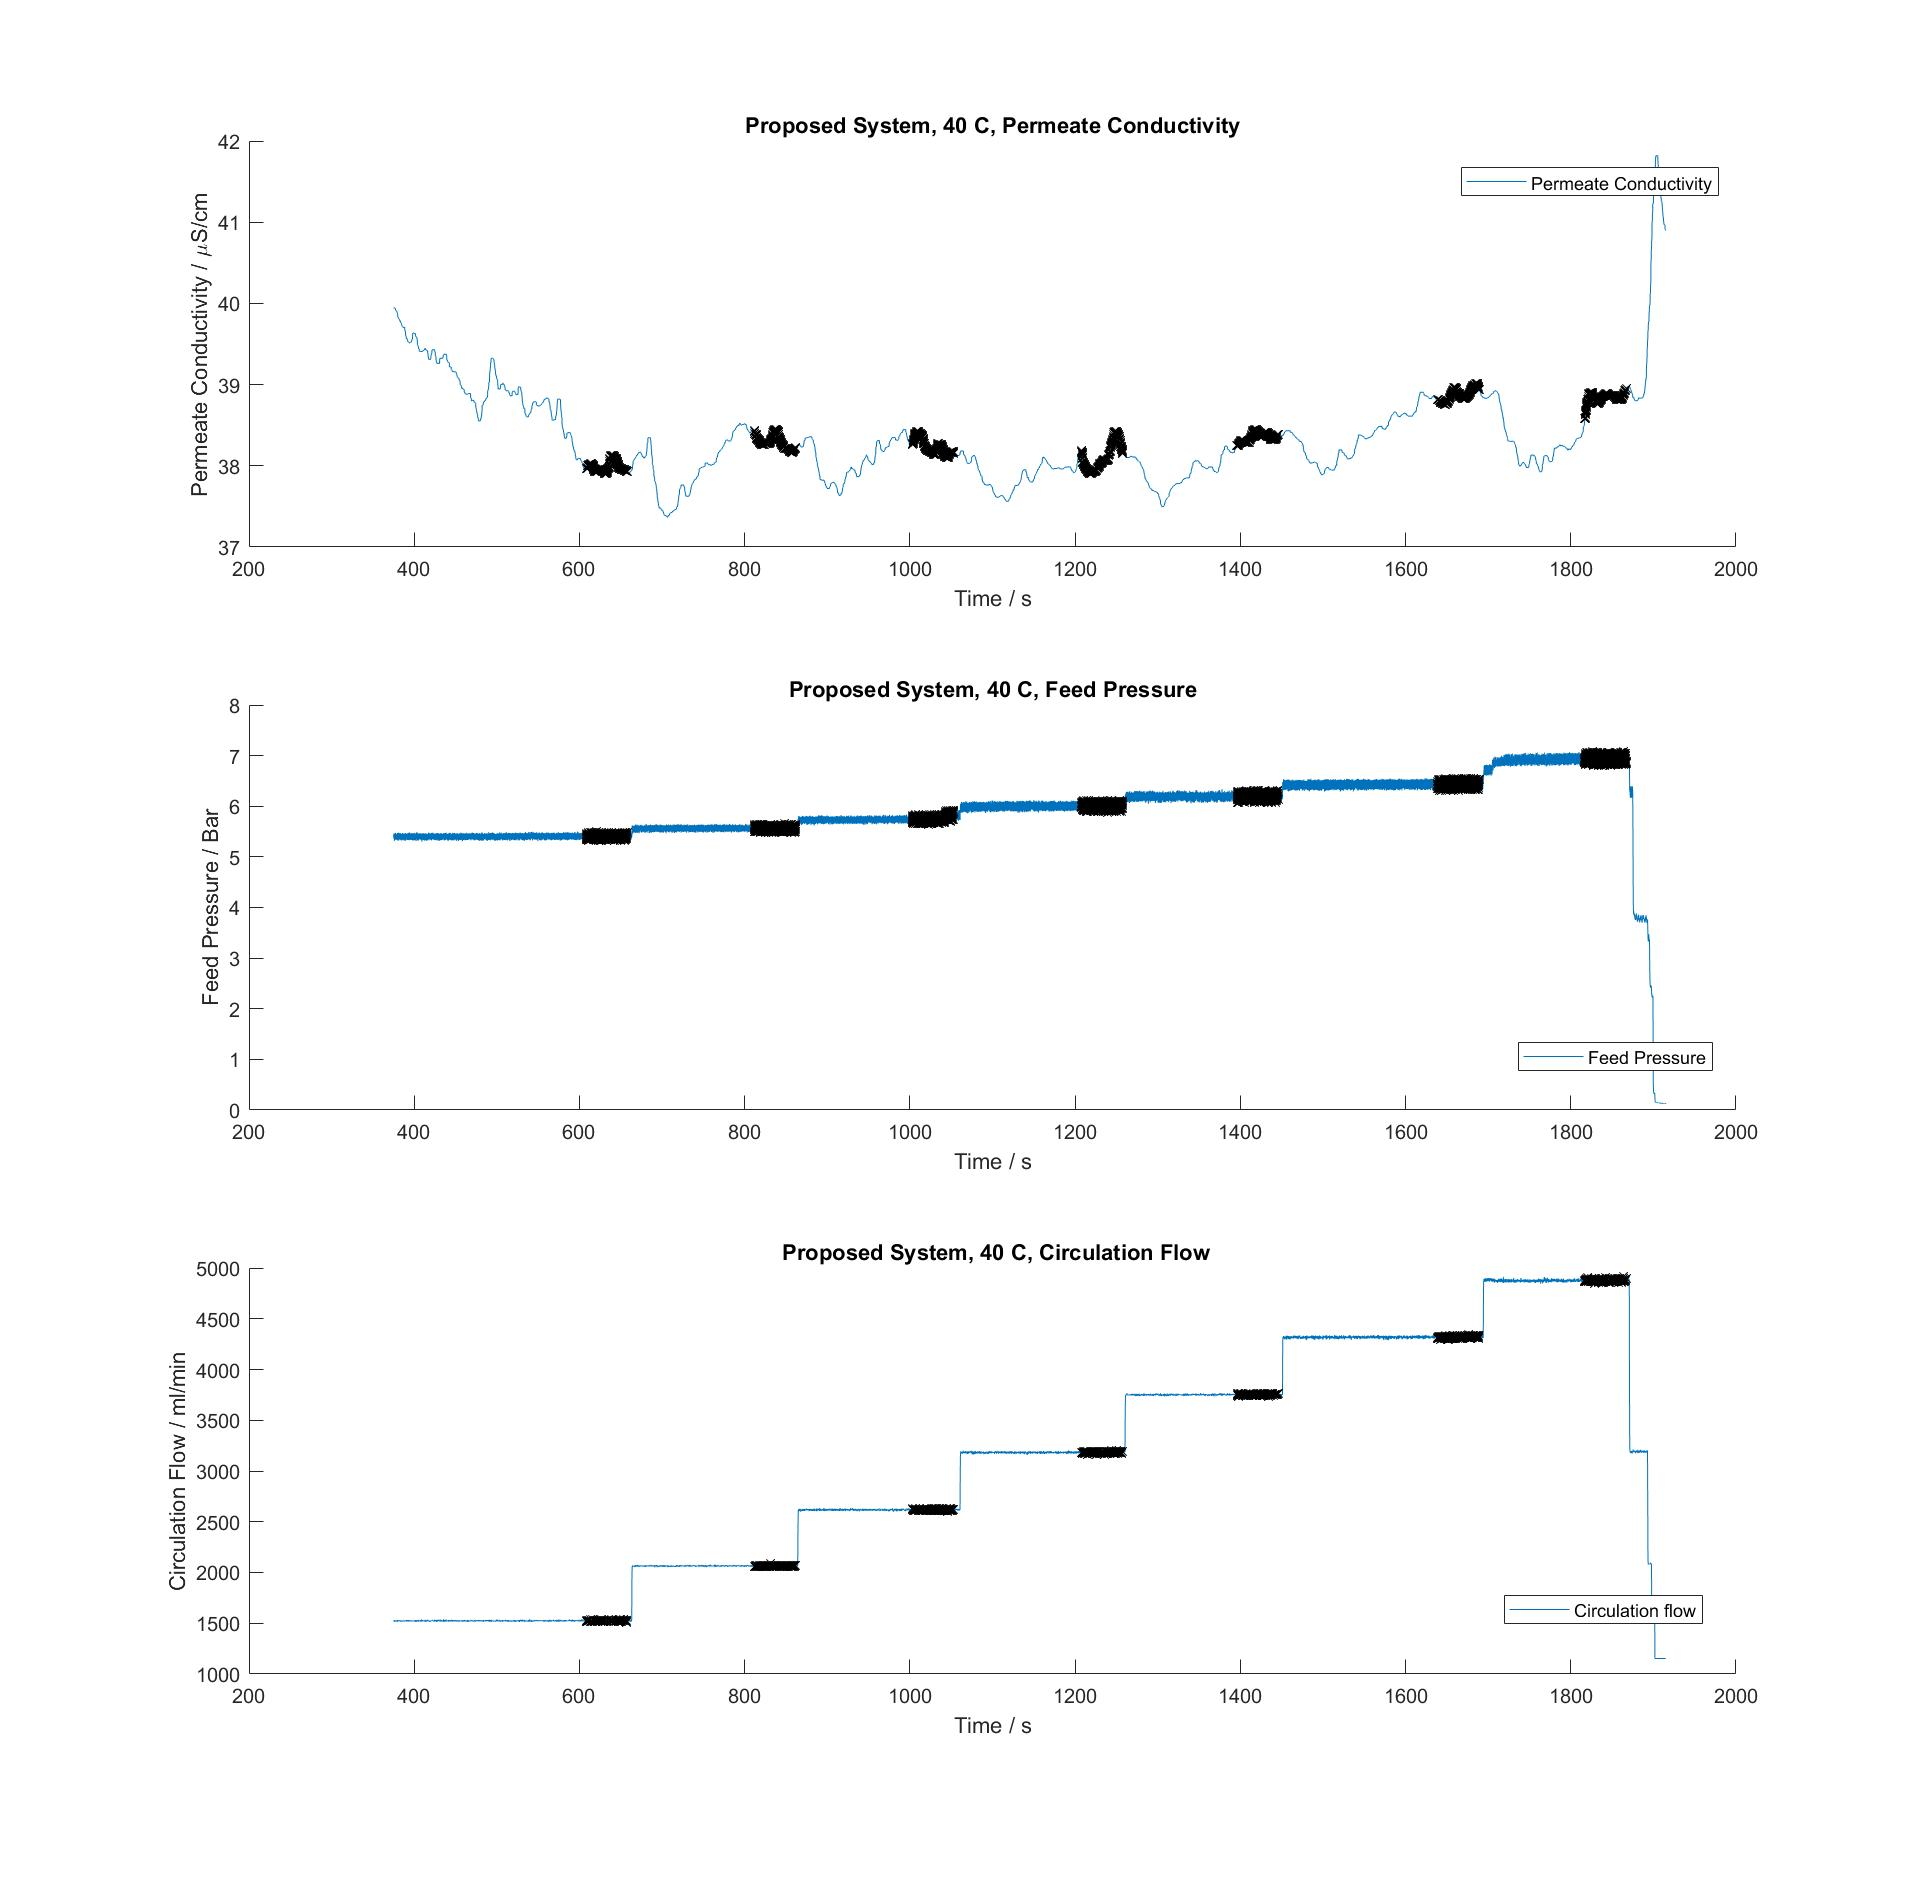
\includegraphics[width=1.1\textwidth]{RecIncrease40}
    \caption{Connections Pressure sensors}
    \label{fig:PressConn}
\end{figure}

\begin{figure}[H]
    \centering
    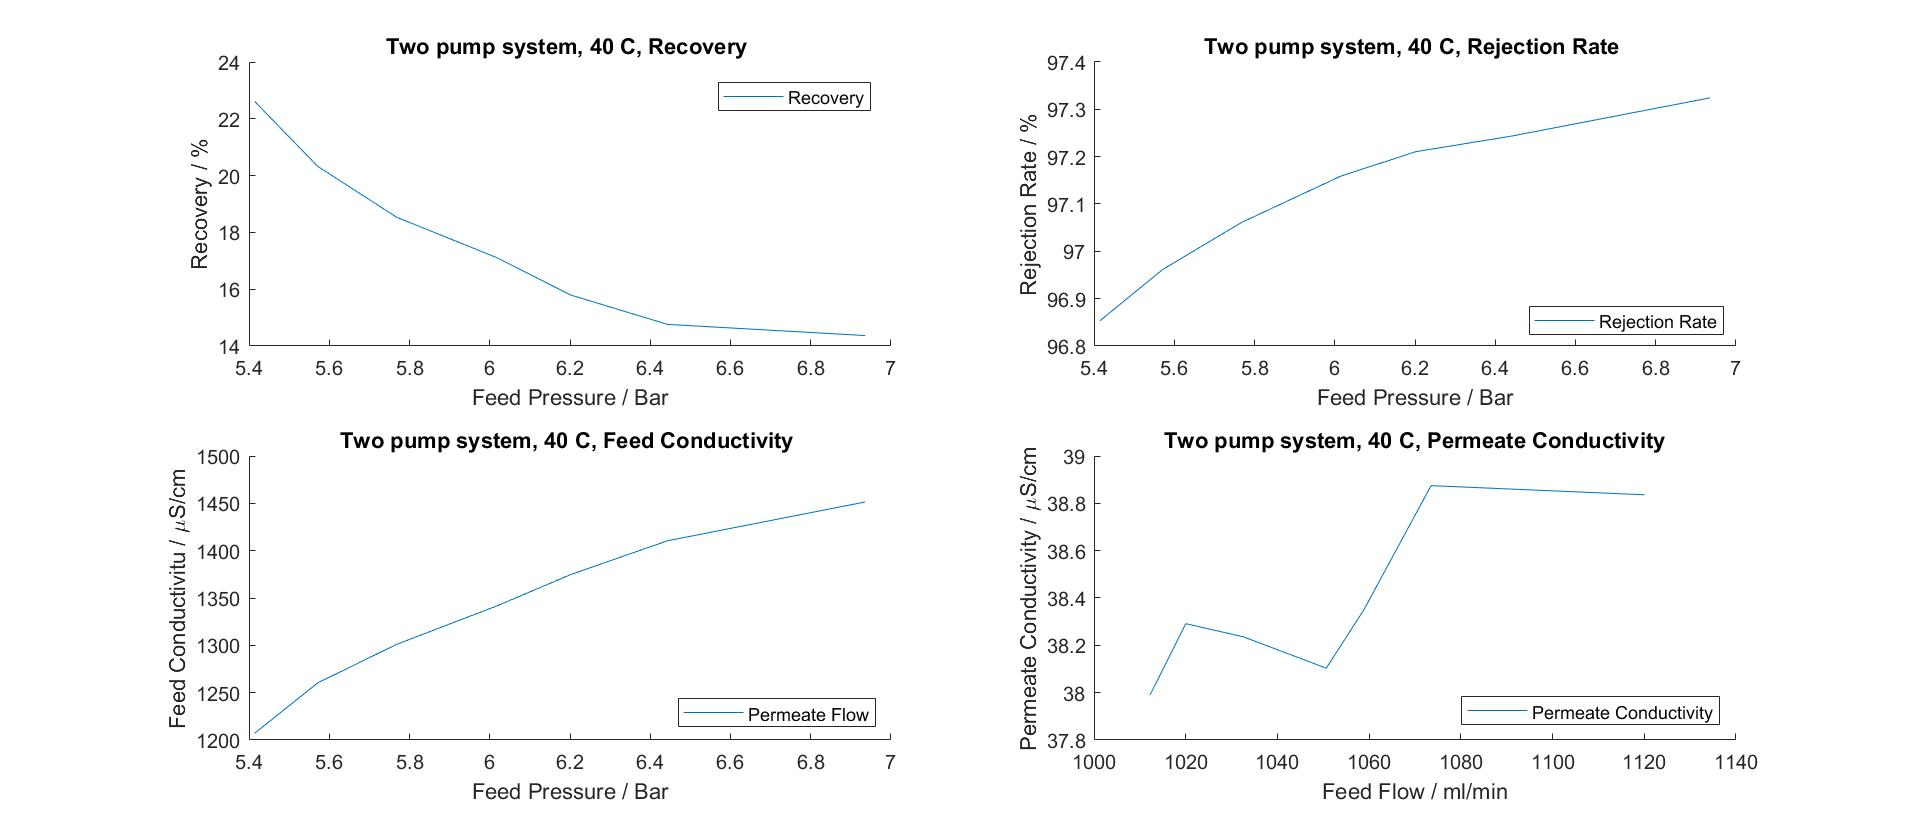
\includegraphics[width=1.1\textwidth]{RecIncrease40Key}
    \caption{Connections Pressure sensors}
    \label{fig:PressConn}
\end{figure}








\section{Modeling}
A physical model of the membrane were made and the given results can be seen in: 

\section{Implementation Test Rig}


\subsection{Connections}
In Figure (\ref{fig:PressConn}-\ref{fig:PumpConn}) all connections in the test rig is displayed.


\begin{figure}[h]
    \centering
    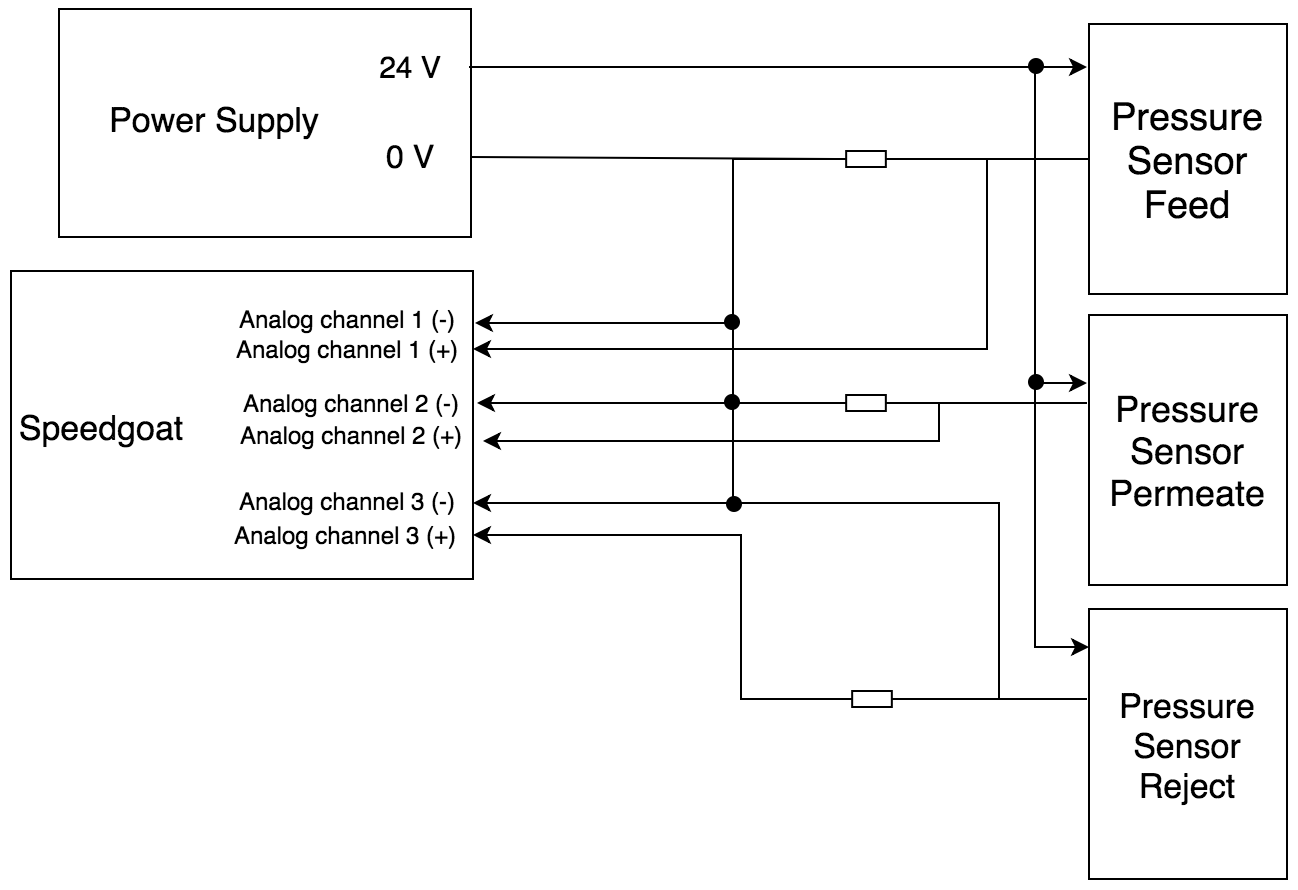
\includegraphics[width=0.7\textwidth]{PressConn}
    \caption{Connections Pressure sensors}
    \label{fig:PressConn}
\end{figure}

\begin{figure}[h]
    \centering
    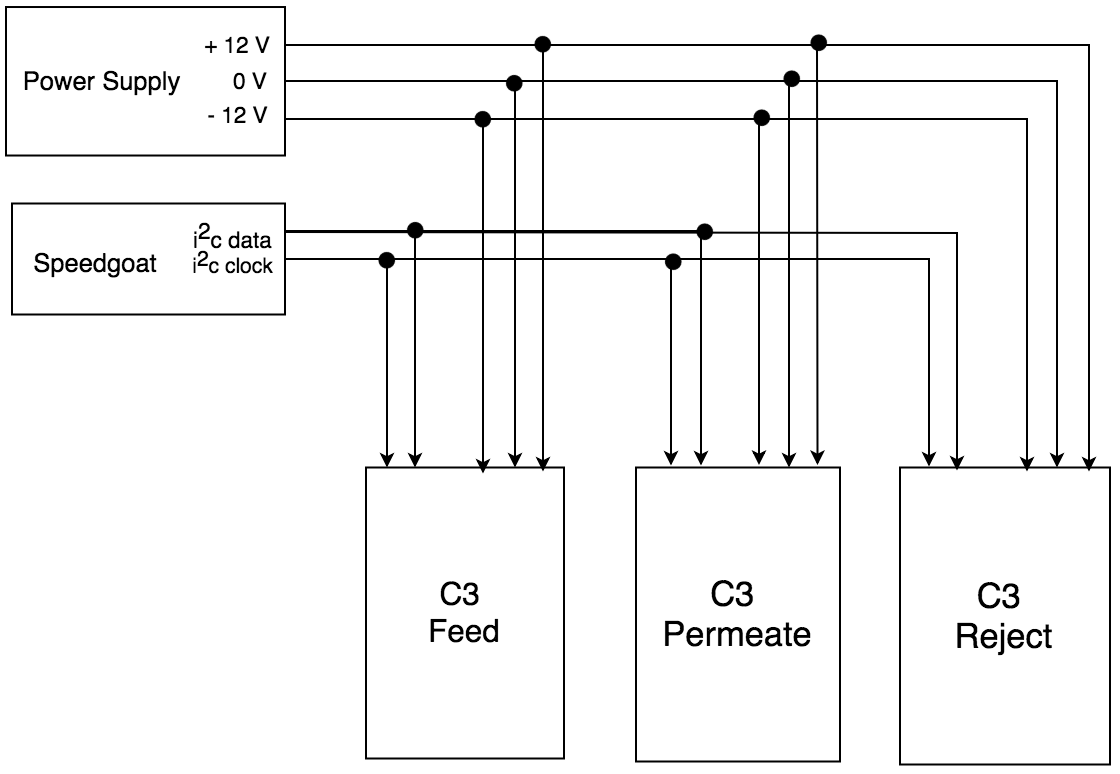
\includegraphics[width=0.7\textwidth]{C3Conn}
    \caption{Connections measurement blocks, C3}
    \label{fig:C3Conn}
\end{figure}

\begin{figure}[h]
    \centering
    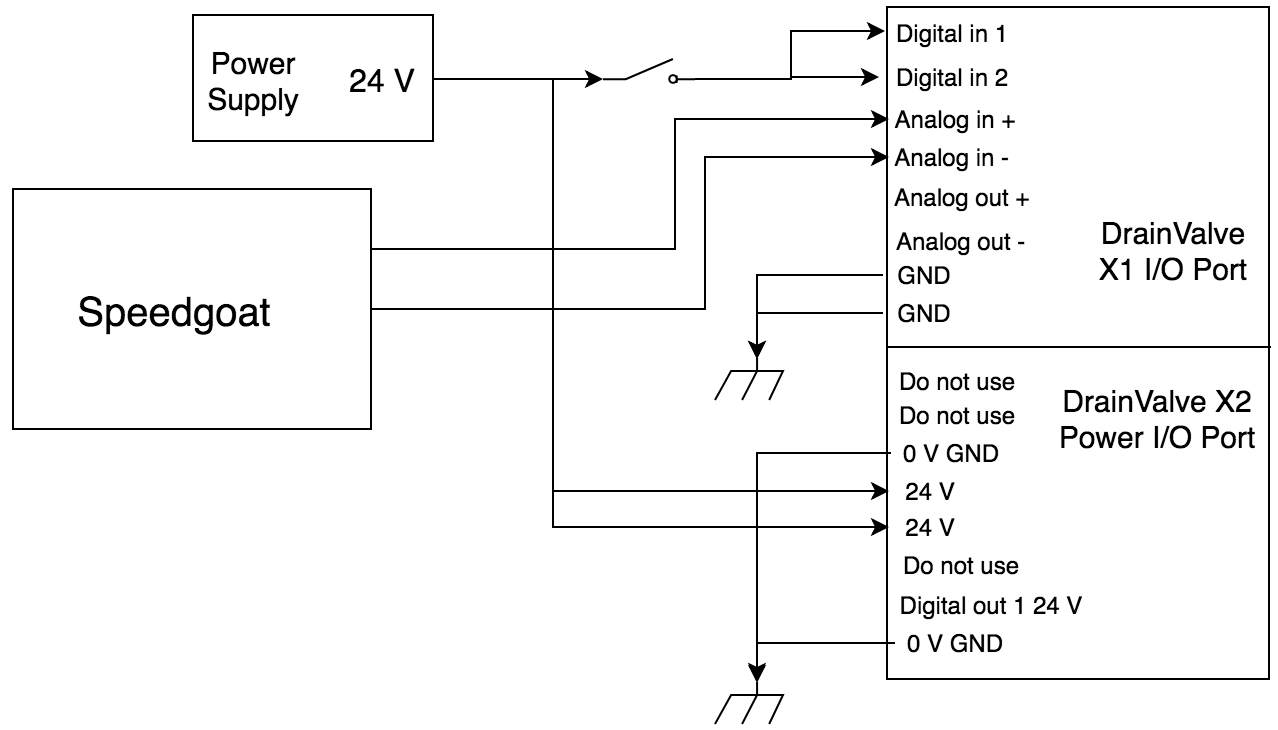
\includegraphics[width=0.7\textwidth]{ValveConn}
    \caption{Connections Drain Valve}
    \label{fig:ValveConn}
\end{figure}

\begin{figure}[h]
    \centering
    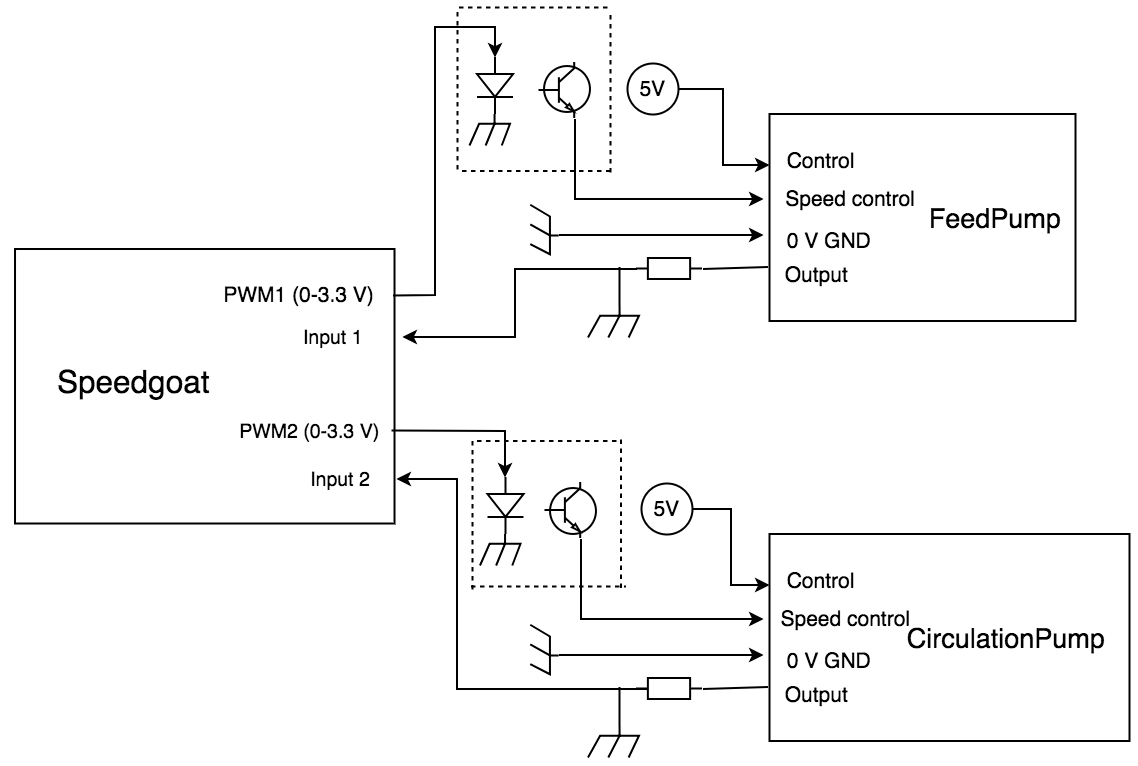
\includegraphics[width=0.7\textwidth]{PumpConn}
    \caption{Connections pumps}
    \label{fig:PumpConn}
\end{figure}


\section{Mapping}
\begin{figure}[h]
    \centering
    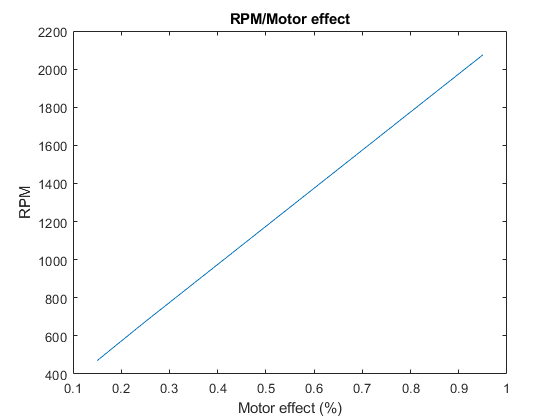
\includegraphics[width=0.7\textwidth]{RPM.png}
    \caption{RPM Pumps}
    \label{fig:RPM}
\end{figure}


\begin{figure}[h]
    \centering
    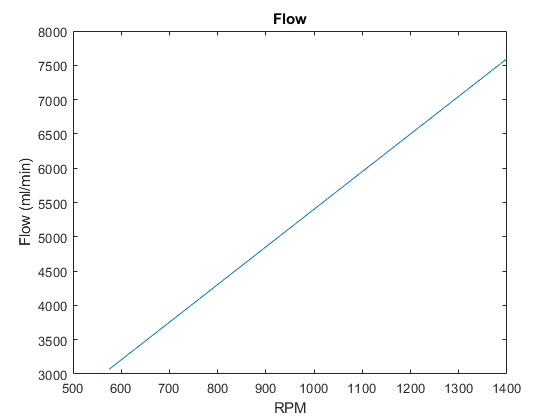
\includegraphics[width=0.7\textwidth]{Flow.png}
    \caption{Flowrate}
    \label{fig:Flowrate}
\end{figure}


\section{Design of control algorithms}

\begin{figure}[h]
    \centering
    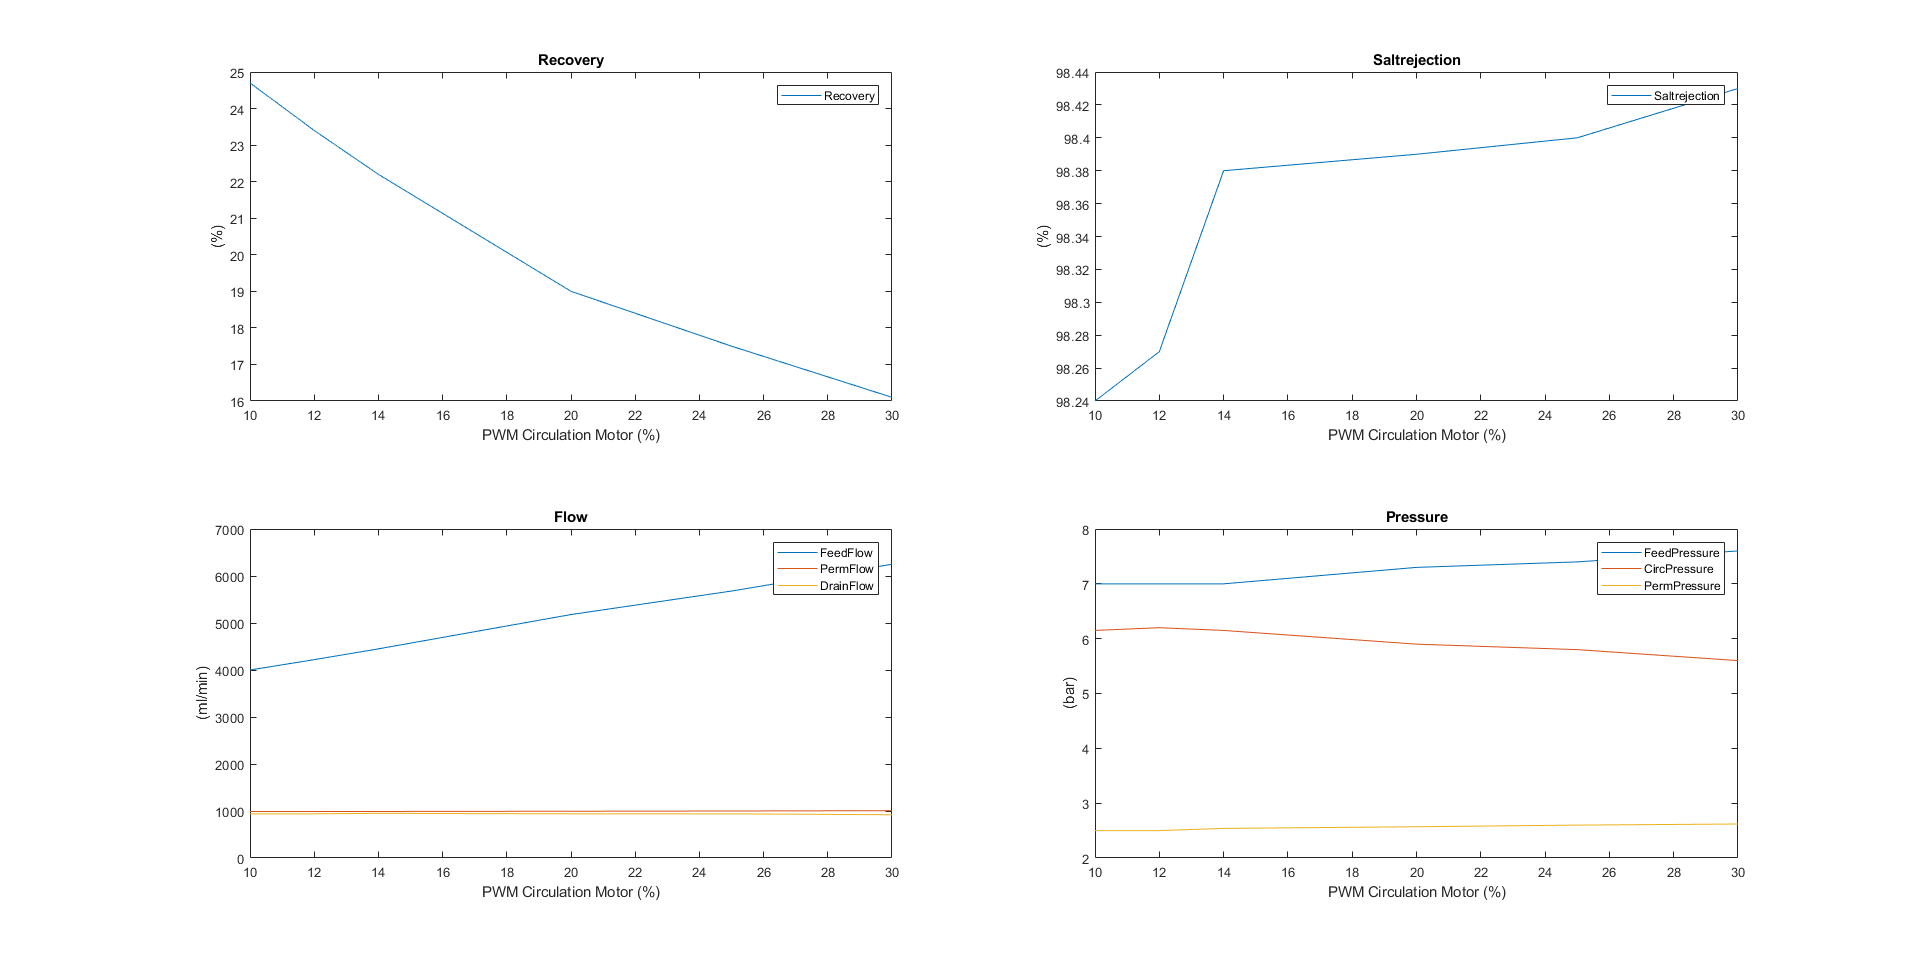
\includegraphics[width=1.65\textwidth, angle = 270]{PreTestReg1.png}
    \caption{Tests with recycle pump as changing parameter}
    \label{fig:PreTestReg1}
\end{figure}

\begin{figure}[h]
    \centering 
    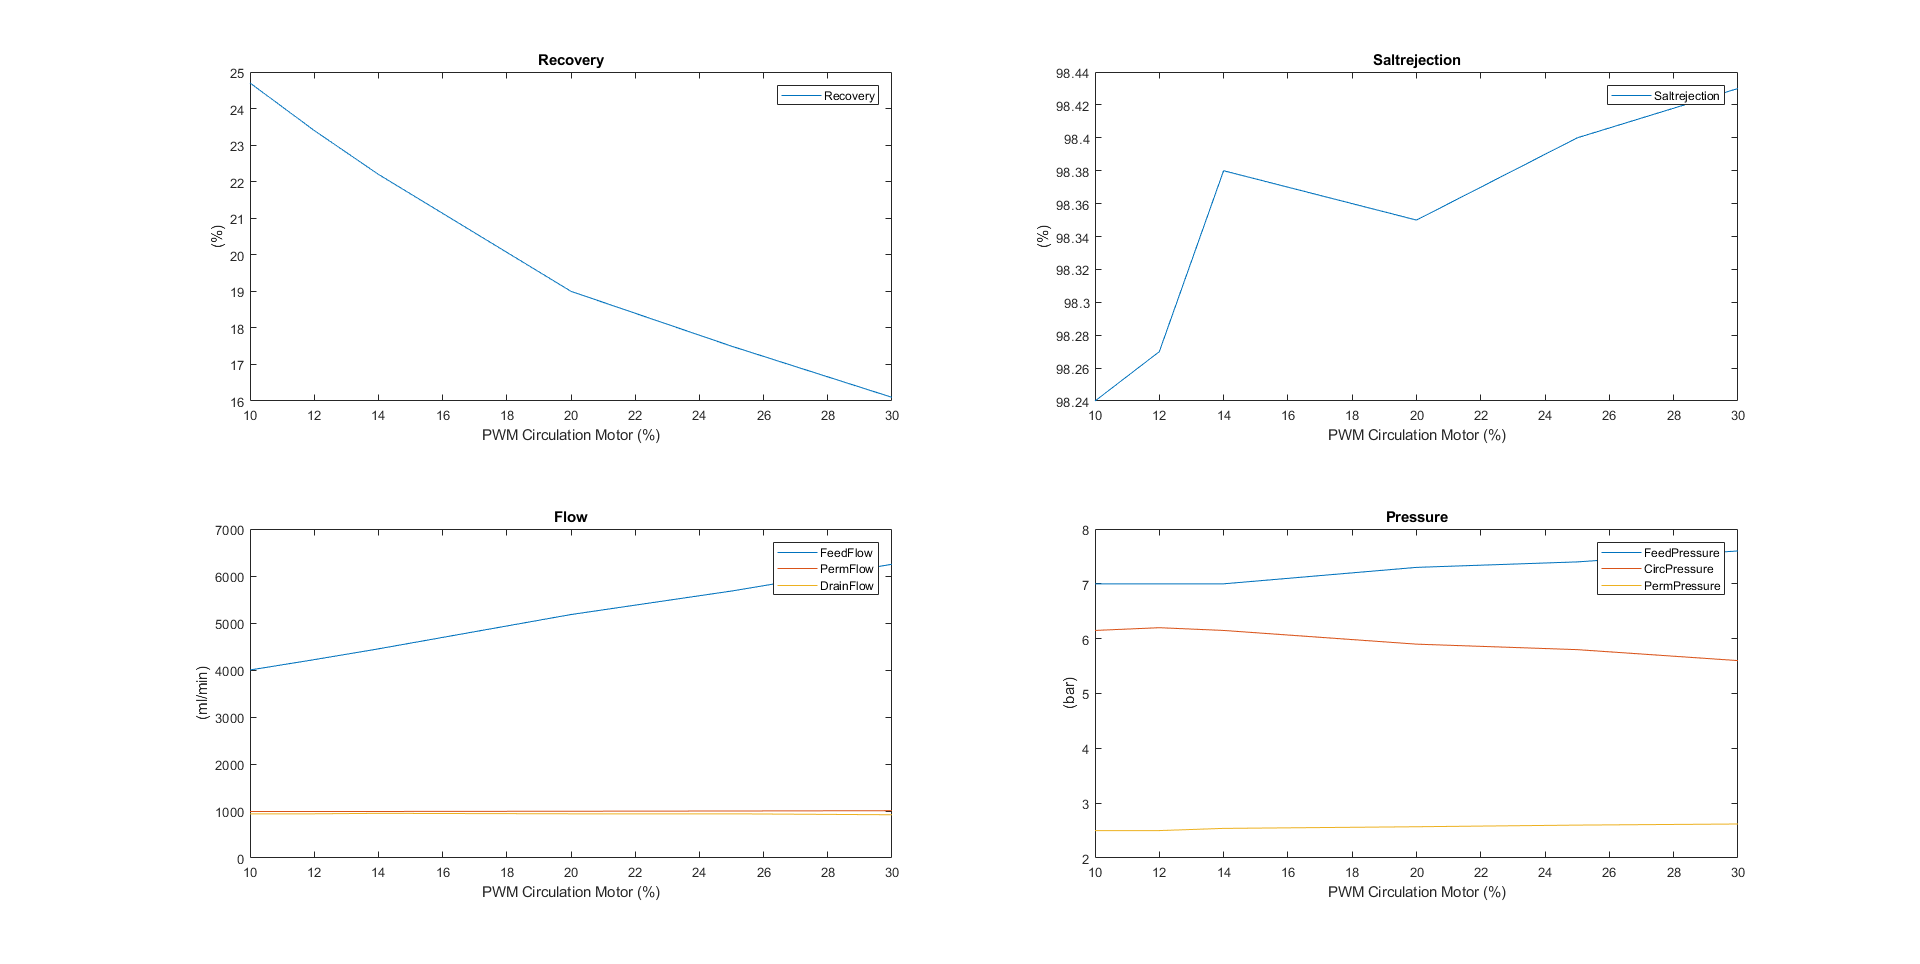
\includegraphics[width=1.65\textwidth, angle=270]{PreTestReg3.png}
    \caption{Tests with inlet pump as changing parameter}
    \label{fig:PreTestReg3}
\end{figure}





FIGURES AND PLOTS FROM SIMSCAPE


\section{Control simulations}




\section{Improvements}
